% EDIT HERE: complete main paper, including all tables, figure layouts and captions.
% References: main.bib.
% Official CVPR2027-v1 author kit; teaser uses the official strip pattern.
\documentclass[10pt,twocolumn,letterpaper]{article}
% Lossless export: compress PDF objects and retain full-resolution visible pixels.
\ifdefined\pdfminorversion\pdfminorversion=7\fi
\ifdefined\pdfcompresslevel\pdfcompresslevel=9\fi
\ifdefined\pdfobjcompresslevel\pdfobjcompresslevel=3\fi
\usepackage[review]{cvpr}
% ===== BEGIN preamble =====
% Explicit dependencies used by the manuscript (not reviewer-facing definitions).
\usepackage{graphicx}
\usepackage{amsmath}
\usepackage{amssymb}
\usepackage{booktabs}
\usepackage{microtype}
\usepackage{placeins}

\usepackage{graphicx}
\usepackage{xcolor}


\usepackage{cuted} % Official two-column teaser support.
% Retain annotation helpers for working copies; no annotation is used in the main text.
\newcommand{\red}[1]{{\color{red}#1}}
\newcommand{\todo}[1]{{\color{red}#1}}
\newcommand{\TODO}[1]{\textbf{\color{red}[TODO: #1]}}
\usepackage{colortbl}
\definecolor{oursbg}{RGB}{236,236,236} % light-gray background of our rows
\definecolor{resultgold}{RGB}{153,117,16}
\definecolor{resultgray}{RGB}{95,102,110}
\newcommand{\na}{\textcolor{black!40}{n/a}}
\newcommand{\nev}{\textcolor{black!40}{--}}
\usepackage{xspace}
\newcommand{\ours}{DynaState\xspace}
\newcommand{\tgroup}[2]{\multicolumn{#1}{@{}l}{\textit{#2}}\\}
% Result-table helpers: shaded "Ours" cells (the group-label column stays unshaded).
\newcommand{\oursname}{\cellcolor{oursbg}\textbf{Ours}}
\newcommand{\ob}[1]{\cellcolor{oursbg}\textbf{#1}}
\newcommand{\oc}[1]{\cellcolor{oursbg}#1}
\newcommand{\hdr}[2]{{\renewcommand{\arraystretch}{0.9}\begin{tabular}[b]{@{}c@{}}#1\\#2\end{tabular}}}

\usepackage{pifont} % check and cross marks for the capability table
\usepackage{tikz}   % half-filled circle for partial support
\definecolor{capgreen}{RGB}{46,125,50}
\definecolor{capgreen}{RGB}{46,125,50}
\definecolor{capamber}{RGB}{222,140,22}
\DeclareRobustCommand{\capyes}{\textcolor{capgreen}{\ding{51}}}
\DeclareRobustCommand{\capno}{\textcolor{black!28}{\ding{55}}}
\DeclareRobustCommand{\cappart}{\tikz[baseline=-0.6ex]{\draw[capamber,line width=0.5pt] (0,0) circle (0.42em);\fill[capamber] (0,0.42em) arc (90:270:0.42em) -- cycle;}}

% Table shading represents rank, independently of method identity.
\definecolor{rankbest}{RGB}{205,225,250}
\definecolor{ranksecond}{RGB}{240,246,253}
\newcommand{\rankbestcell}[1]{\begingroup\setlength{\fboxsep}{1.5pt}\colorbox{rankbest}{\kern1.2pt\textbf{#1}\kern1.2pt}\endgroup}
\newcommand{\ranksecondcell}[1]{\begingroup\setlength{\fboxsep}{1.5pt}\colorbox{ranksecond}{\kern1.2pt#1\kern1.2pt}\endgroup}
\newcommand{\ranklegend}{\begingroup\setlength{\fboxsep}{0.7pt}\colorbox{rankbest}{best}/\colorbox{ranksecond}{second}\endgroup}
% ===== END preamble =====
% ===== BEGIN draft_macros =====
% Draft markers for the Method/Experiments drafts (draft-marker-discipline).
% \TODO       an unresolved factual or sourcing question (a number, a run, a protocol)
% \note       editorial remark addressed to the authors
% \directive  a change this passage must receive, and why
% \superseded text replaced by a decision, kept visible in draft mode
% Set \draftmodefalse to hide all four for a clean copy.
% The manuscript preamble already defines \TODO; \providecommand keeps that definition.
\usepackage{xcolor}
% Temporary author-discussion highlights. Set \discussionmarksfalse for a clean copy.
\newif\ifdiscussionmarks
\discussionmarkstrue
\DeclareRobustCommand{\discuss}[1]{\ifdiscussionmarks\textcolor{red!70!black}{#1}\else#1\fi}

\usepackage{multirow}
\newif\ifdraftmode
\draftmodetrue
\providecommand{\TODO}[1]{\textbf{\color{red}[TODO: #1]}}
% \prov{x}   a provisional number: the best value available now, to be replaced by the final runs (source in the
%            % SRC comment next to it). Draft mode prints it in brown; clean mode prints it plainly.
% \pend      a table cell whose run or scoring is still pending: a red dash in draft mode, -- in the clean copy.
\ifdraftmode
  \newcommand{\prov}[1]{{\color{brown}#1}}
  \newcommand{\pend}{{\color{red}--}}
  \newcommand{\note}[1]{{\color{blue}[Note: #1]}}
  \newcommand{\directive}[1]{\par\noindent\fbox{\parbox{0.95\linewidth}{\small\textbf{Directive:} #1}}\par}
  \newcommand{\superseded}[1]{{\color{gray}#1}}
\else
  \newcommand{\prov}[1]{#1}
  \newcommand{\pend}{\nev}
  \renewcommand{\TODO}[1]{}
  \newcommand{\note}[1]{}
  \newcommand{\directive}[1]{}
  \newcommand{\superseded}[1]{}
\fi
% ===== END draft_macros =====
\definecolor{cvprblue}{rgb}{0.21,0.49,0.74}
\usepackage[pagebackref,breaklinks,colorlinks,allcolors=cvprblue]{hyperref}
\def\confName{CVPR}
\def\confYear{2027}
\title{DynaState: Unified Dynamic Mapping within and across Visits}
\author{Anonymous Authors}
\begin{document}
\maketitle
% ===== BEGIN figures / teaser_front =====
\begin{strip}
\centering
\vspace{-10mm}
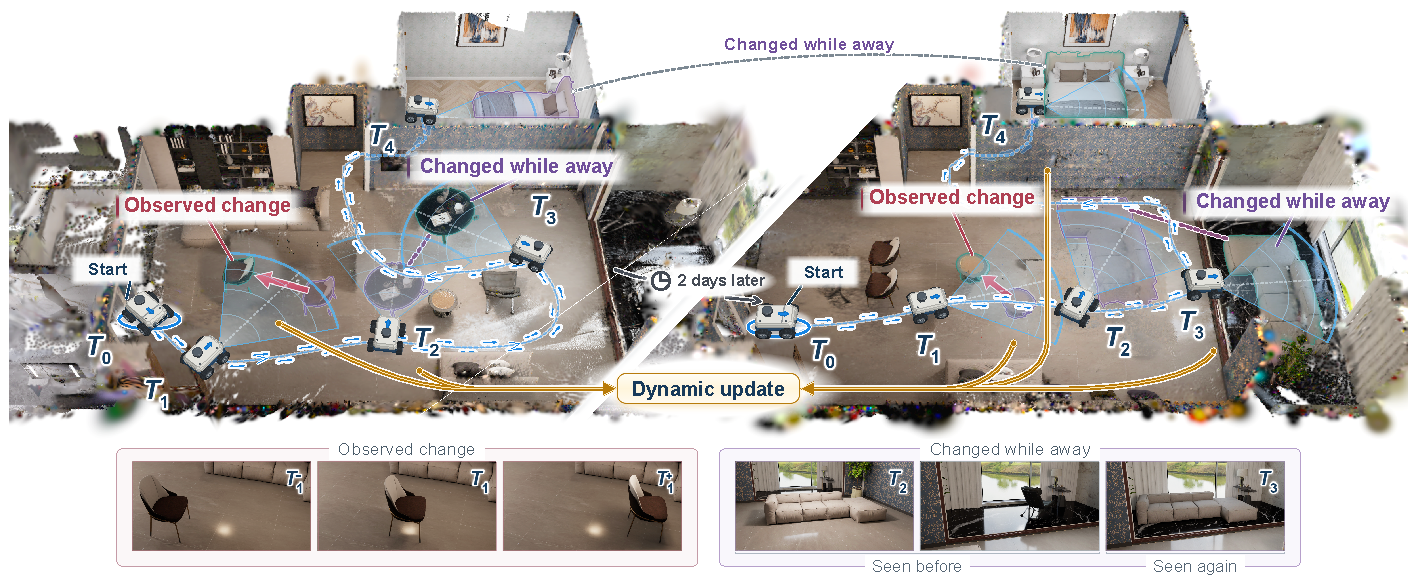
\includegraphics[width=\linewidth]{figures/export_lossless/teaser_with_zooms.pdf}
\vspace{-5mm}
\captionsetup{hypcap=false}
\captionof{figure}{\textbf{One map follows scene changes within and across visits.} A robot sees objects move (red)
and later discovers, after looking away or after returning days later, that objects are missing or new (purple).
Both lead to the same dynamic update: the ended object states are retired together with their unseen parts, the
changed scene is reconstructed, and earlier geometry that is still valid is kept. Every element carries a lifetime,
so the map can also be queried at any past time.}
\label{fig:teaser}
\captionsetup{hypcap=true}
\end{strip}
% ===== END figures / teaser_front =====
% ===== BEGIN sec / 0_abstract =====
\begin{abstract}
Robots working in human spaces over weeks need a 3D map that updates what changes, keeps what persists, and recalls past
layouts. Objects move in view, shift out of view, and rearrange across visits, yet prior mappers handle isolated cases:
keeping old frames of a moved chair re-fuses it and carves away newcomers, whereas dropping them loses static walls.
Here we introduce \ours, where one decision resolves both conflicts by starting or ending an object state,
confirmed by surface-coverage evidence from partial views. It retires ended geometry, unseen parts included, to
queryable history and limits past observations to the states and regions they still describe. Acting on states, not
voxels, splats, or cells, one method drives TSDF, 3D Gaussian, and occupancy maps alike. In each representation,
\ours beats the strongest map-specific baseline (Khronos, GaME, Wavemap) in mesh, object, and change F1 on public
benchmarks and our new one, with up to $2.4\times$ change F1 and +3.9\,dB PSNR. The code and data will be released.
\end{abstract}
% ===== END sec / 0_abstract =====
% ===== BEGIN sec / 1_intro =====
\section{Introduction}
\label{sec:intro}

The world does not reset when a mapper restarts. Objects move in front of a robot, shift while it looks elsewhere, and
rearrange between visits (\cref{fig:teaser}). These changes pose a central challenge for lifelong mapping: maintaining one consistent map within and across visits that updates what changes, retains what persists, and supports historical queries.

Existing mappers solve fragments of this problem within isolated representations (\cref{tab:capabilities}).
Khronos~\cite{Schmid-RSS-24} tracks visible motion and checks object absence within a TSDF session. Panoptic
Multi-TSDFs~\cite{9811877} and POCD~\cite{Qian-RSS-22} reason about object persistence across TSDF scans while leaving
in-view motion aside. GaME~\cite{Yugay_2026_CVPR}, CL-Splats~\cite{Ackermann_2025_ICCV}, and
GaussianUpdate~\cite{Zeng_2025_ICCV} adapt 3D Gaussian maps across captures, and Wavemap~\cite{Reijgwart-RSS-23}
overwrites occupancy cells through clamped log-odds. Once a scene changes, all face the same dilemma: earlier frames of
a removed chair would fuse the chair back, their free-space rays would carve away a sofa placed in its spot, and their
keyframes would train Gaussians for a vanished layout, yet those same frames also observed the unchanged static objects. GaME expands removal through historical object masks and masks stale keyframe regions,
while volumetric systems update object submaps and free-space evidence.
They address the conflict within individual representations. A past observation can become invalid for a changed object while remaining valid for unchanged surfaces.
We seek one change decision that governs both geometry and observation contributions across representations.

We treat every discrete scene change as a transition of \emph{object state}. An object holds one configuration over a
half-open time interval. Its geometry belongs in the map during that interval, and each observation constrains only the
states it recorded. Ending/starting a state thus determines both geometry and observation validity. When the
chair's state ends, its entire surface retires from the current map, unseen back included. Rays in earlier frames that
hit the chair stop contributing to the current volume, whereas rays that hit the wall behind it keep their surface band
but stop their free space before the newly arrived sofa. Surface evidence confirms the change from partial views,
and the resulting state transition governs both operations within and across visits.
DynaState maintains object states across visits
and unifies state transitions across TSDF, Gaussian,
and occupancy maps. Each transition governs both geometry
and observation validity, preventing historical
observations from corrupting the updated map.


Since public datasets isolate either in-view motion or cross-visit changes, we introduce \emph{DynaState-Real} and
\emph{DynaState-Sim}, an RGB-D benchmark combining in-view motion, out-of-view changes, and multi-visit rearrangements
in a single map, and evaluate further on Flat~\cite{9811877}, 3RScan~\cite{9010673}, TESSE~\cite{Schmid-RSS-24}, and
Aria~\cite{Pan_2023_ICCV,Yugay_2026_CVPR}. Across Real, Sim, Flat, and 3RScan, \ours improves mesh, object, and change
F1 over the native update of all three representations. On TESSE, change F1 rises from 46.2 to 78.6 in Office and from
38.6 to 92.6 in Apartment. On a partial revisit in Sim, continuing our TSDF map improves mesh F1 by 9.3 points over
restarting our mapper and by 12.6 points over restarting Khronos. On Flat and Aria, our Gaussian maps exceed GaME by
0.88--3.91\,dB PSNR.

\vspace{1mm}\noindent\textbf{Contributions:}
\begin{itemize}
  \item \textbf{Unified dynamic mapping:} We formulate changes within and across visits as object-state
  transitions that jointly govern geometry and observation validity across TSDF, Gaussian, and occupancy maps.
  \item \textbf{Representation-agnostic observation validity:} We bound historical observation influence via volumetric
  valid domains and capture-time Gaussian keyframes, driving TSDF, 3DGS, and occupancy with their native
  integration rules kept intact.
  \item \textbf{Joint dynamic benchmark and evaluation:} We release DynaState-Real and DynaState-Sim, uniting in-view,
  out-of-view, and cross-visit changes, and demonstrate consistent gains across six benchmarks.
\end{itemize}

% ===== BEGIN tables / capabilities =====
\begin{table*}[t]
\centering
\small
\setlength{\tabcolsep}{4pt}
\renewcommand{\arraystretch}{1.2}
\begin{tabular}{llcccccc}
\toprule
& & \multicolumn{3}{c}{\textbf{Changes handled}} & \multicolumn{3}{c}{\textbf{Map properties}} \\
\cmidrule(lr){3-5}\cmidrule(lr){6-8}
Method & Representation & \hdr{In}{view} & \hdr{After}{looking away} & \hdr{Across}{visits} & \hdr{Observation}{validity} & \hdr{Historical}{queries} & \hdr{Novel-view}{synthesis} \\
\midrule
Panoptic Multi-TSDFs~\cite{9811877} & TSDF & \capno & \capyes & \capyes & \cappart & \cappart & \capno \\
POCD~\cite{Qian-RSS-22} & TSDF & \capno & \capyes & \capyes & \cappart & \capno & \capno \\
Khronos~\cite{Schmid-RSS-24} & TSDF & \capyes & \cappart & \cappart & \capno & \capyes & \capno \\
\addlinespace[2pt]
CL-Splats~\cite{Ackermann_2025_ICCV} & 3DGS & \capno & \cappart & \capyes & \cappart & \capyes & \capyes \\
GaussianUpdate~\cite{Zeng_2025_ICCV} & 3DGS & \capno & \cappart & \capyes & \cappart & \cappart & \capyes \\
GaME~\cite{Yugay_2026_CVPR} & 3DGS & \capno & \cappart & \cappart & \cappart & \capno & \capyes \\
\addlinespace[2pt]
Wavemap~\cite{Reijgwart-RSS-23} & Occupancy & \cappart & \cappart & \cappart & \capno & \capno & \capno \\
\midrule
\rowcolor{oursbg}
\textbf{Ours} & TSDF, 3DGS, Occupancy & \capyes & \capyes & \capyes & \capyes & \capyes & \capyes$^{\dagger}$ \\
\bottomrule
\end{tabular}
\caption{\textbf{Mapping capabilities.} \capyes{} supported, \cappart{} partial, \capno{} not supported. In view:
moving objects are detected and reconstructed once they settle. After looking away: full when a change found
within a run retires the whole object, partial when only the re-observed part is updated. Across visits: full
when map and object states continue into a later visit, partial when visits are concatenated into one run or
states are not carried. Observation validity: full when earlier observations are restricted per state and
region, partial when whole submaps or keyframes are frozen or set aside. Historical queries: full when the map
can be queried at past times, partial when past objects are kept without time stamps. $^{\dagger}$Novel views
come from the 3DGS branch.}
\label{tab:capabilities}
\end{table*}
% ===== END tables / capabilities =====
% ===== END sec / 1_intro =====
% ===== BEGIN sec / 2_related_work =====
\section{Related Work}
\label{sec:related_work}

\noindent\textbf{Dense map representations.}
Dense mapping uses signed-distance volumes~\cite{10.1145/237170.237269,6162880,8202315}, surfel
meshes~\cite{schops2020surfelmeshing}, and probabilistic occupancy~\cite{10.1007/s10514-012-9321-0,Reijgwart-RSS-23}.
Gaussian splatting~\cite{10.1145/3592433} supports joint camera tracking, mapping, and rendering in MonoGS and
SplaTAM~\cite{Matsuki_2024_CVPR,Keetha_2024_CVPR}. Each of them integrates a measurement in its own way, by weighted
averaging of signed distances, by log-odds updates, or by gradient steps on a rendering loss. We keep these
integrations unchanged and govern all of their map updates online through shared object states and element lifetimes.

\vspace{1mm}\noindent\textbf{Dynamic reconstruction.}
WildGS-SLAM reconstructs the static surroundings by suppressing moving regions~\cite{Zheng_2025_CVPR}. Co-Fusion,
MID-Fusion, and EM-Fusion reconstruct objects while they move~\cite{7989518,8794371,9010932}, and DynaSLAM~II and
DynoSAM estimate camera and object motion jointly~\cite{9385844,11288097}. Dynablox detects moving points as those
that fall into space known to be free, without any prior on object appearance~\cite{10218983}. Dynamic Gaussian
methods model motion and deformation~\cite{Matsuki_2025_CVPR,Li_2025_ICCV,Li_2026_WACV,Wang_2026_CVPR}, and 4D
Primitive-M\^ach\'e assembles observations across time into persistent reconstructions~\cite{Mazur_2026_CVPR}.
Spacetime Gaussians and 4D Gaussian splatting give each Gaussian a temporal opacity learned from a complete
capture~\cite{Li_2024_CVPR_spacetime,Wu_2024_CVPR_4dgs}, the nearest relative of our element lifetimes, which are
decided online. These methods model motion while it is observed. A change that happens out of view leaves no
motion to track. We use the free-space cue of Dynablox to detect visible motion and treat the settled object as a
new state, so a change observed in motion and a change discovered only after the fact both enter the very same
state-transition mechanism.

\vspace{1mm}\noindent\textbf{Updating evolving scenes.}
Long-term map maintenance updates point clouds~\cite{6907397,8594310,9811916,10802029} and volumetric
surfaces~\cite{7989614,9811877}. Removert and ERASOR build static LiDAR maps by removing points that later scans
see through~\cite{kim2020removert,lim2021erasor}, the cue behind our see-through evidence, applied per point and
without object states. Panoptic Multi-TSDFs freezes inactive object submaps and marks a submap absent once 20
of its surface points, or 2\%, conflict with the active submaps, while objects moving in view are left to future
work~\cite{9811877}. POCD estimates object change and stationarity, and POV-SLAM couples this reasoning with pose
estimation~\cite{Qian-RSS-22,Qian-RSS-23}. Khronos combines motion detection with absence verification against
the rays stored for each observation, confirms absence once 60\% of the rays in a 5\,s window agree, and keeps
every object fragment together with an estimated presence interval in a map that remains queryable over
time~\cite{Schmid-RSS-24}.

For Gaussians, LT-Gaussian and GaussianUpdate maintain maps through scene changes~\cite{11097624,Zeng_2025_ICCV},
and CL-Splats updates local regions from sparse captures and recovers earlier states~\cite{Ackermann_2025_ICCV}.
SynGS learns per-Gaussian change probabilities together with illumination-aware updates~\cite{huang2025syngs}, O-SCD
fuses multi-view change cues online~\cite{galappaththige2026changes}, and 3DGS-CD detects object rearrangements from
lifted SAM masks~\cite{Kirillov_2023_ICCV,lu20253dgscd}. GaME detects changes from rendering conflicts, expands
object removal through historical masks, and masks stale keyframe regions. It can exclude a keyframe once one of its
masks is mostly stale~\cite{Yugay_2026_CVPR}. GS-LTS actively acquires views for Gaussian
editing~\cite{fu2025gslts3dgaussiansplattingbased}, and GS-Diff detects changes between Gaussian
reconstructions~\cite{galappaththige2026gsdiff}. These systems decide changes per submap, per ray, or per
Gaussian and then patch the observations with a rule of their own. We decide per object state and carry the
decision, through valid domains and capture-time maps, to every element and every observation in all three
representations.

\vspace{1mm}\noindent\textbf{Object association and scene history.}
RIO re-localizes instances in changed scans~\cite{9010673}, and Living Scenes reconstructs objects across
scans~\cite{Zhu_2024_CVPR}. ObVi-SLAM and OASIS-Map associate object landmarks across
sessions~\cite{10423794,oh2026oasismapobjectlevelchangedetection}, and 3D VSG predicts semantic scene
changes~\cite{10161212}. Persistence models reason about feature survival~\cite{7487237,9196913}, occupancy
transitions~\cite{DBLP:conf/aaai/Meyer-DeliusBB12}, periodicity~\cite{7878680}, or multiple appearance and
disappearance hypotheses~\cite{11247086}. These models estimate whether an object persists. We combine such persistence
priors with observed surface evidence to update both map geometry and observation validity.

% ===== END sec / 2_related_work =====
% ===== BEGIN sec / 4_method =====
\section{Method}
\label{sec:method}

\ours maintains one map within and across visits from posed RGB-D frames with instance masks; semantic masks and
SAM segments~\cite{Kirillov_2023_ICCV} are handled by front-end adaptation. Poses come from a SLAM system or from
the dataset, masks from annotations or from a segmenter, and associations link the masks of one object across frames. Each
change is first judged and then applied to the map (\cref{fig:method}): \emph{change detection} decides from current depth which object states continue, end,
or begin (\cref{sec:states}), and \emph{map update} applies the decision to the stored geometry and to the
observations that keep shaping it (\cref{sec:validity}). Both act on object states and on capture times, so one set of
decisions drives TSDF, Gaussian, and occupancy maps alike (\cref{sec:representations}). One example runs through this
section and \cref{fig:method}: an armchair leaves, a sofa arrives in front of a wall, and the wall stays where it is.

\begin{figure*}[t]
\centering
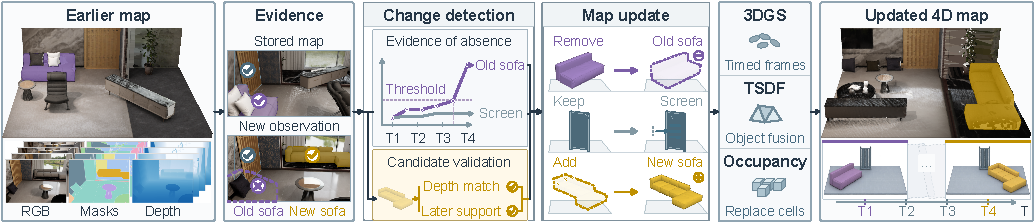
\includegraphics[width=\textwidth]{figures/export_lossless/pipeline_halfgrid_operations.pdf}
\caption{\textbf{A scene change updates both geometry and observation contributions.}
RGB-D frames, masks, and poses provide evidence against the retained map.
Accumulated absence evidence ends the armchair's state (purple), while depth
agreement and later observations validate the new sofa (yellow).
Map update retires the armchair from the current map, keeps the wall,
and adds the sofa. These decisions govern Gaussian, TSDF, and occupancy
updates, while state lifetimes preserve earlier maps for historical queries.}
\label{fig:method}
\end{figure*}

\vspace{1mm}\noindent\textbf{Map representation.}
\label{sec:setting}
A \emph{state} is one configuration of an object; masks and associations group its observations, so further views
complete the surface of the same state. State $s$ has a surface $G_s$ and a \emph{state interval} $[b_s,d_s)$ that
fixes when its geometry belongs in the map and which observations describe it. Each map element $e$, a TSDF face, a
Gaussian, or an occupied cell, carries its object association, if any, and a lifetime $[c_e,d_e)$ that follows its
state. The map at time $t$ is then the set of all elements alive at $t$,
\begin{equation}
  \mathcal{M}(t)=\{e\in\mathcal{E}:c_e\leq t<d_e\}.
  \label{eq:map_at_t}
\end{equation}
Ending a state ends the lifetimes of its elements: the armchair leaves $\mathcal{M}(t)$ for later times and stays
in it for earlier ones. An element allocated later to a continuing state inherits that state's start, not its own
allocation time.

\subsection{Change Detection}
\label{sec:states}

The camera sees only part of an object at a time, and an unseen surface is not a missing one: the armchair may sit
behind the new sofa or out of view. A decision should come as soon as the evidence suffices, yet repeated views of
one patch must not add up to a change of the whole object. One test covers changes in view, after looking away, and
between any two visits.

\vspace{1mm}\noindent\textbf{Surface evidence.}
We project surface samples of $G_s$ into each new depth image. Only reliable samples count, those never seen through
while in place, and only rays below $60^\circ$ incidence see through them, since grazing views of noisy depth
produce false see-through evidence~\cite{6375037}. The depth tolerance equals the voxel or cell
size~\cite{9811877}; Gaussian maps use a 5\,cm reference scale. A sample is \emph{supported} when the depths agree,
\emph{seen through} when the measurement lies farther along the ray, and \emph{occluded} when it lies closer. Seeing
the floor where the armchair stood shows that it has left, whereas the sofa only occludes the wall behind it.
Occlusions, invalid depths, and samples outside the image add no evidence, so an object hidden by
a larger one at the same spot persists until its surroundings reappear.

\vspace{1mm}\noindent\textbf{Change decisions.}
A \emph{round} is a depth image that judges at least $\min(30,\nu_{\mathrm{rel}})$ reliable samples of state $s$,
where $\nu_{\mathrm{rel}}$ is the state's number of reliable samples; the floor of 30 follows the relative-support scale of Panoptic Multi-TSDFs~\cite{9811877}. Let $f_i$ be the fraction of judged samples that round $i$ sees through. While the object
is in place, $f_i$ follows a Beta density fitted to earlier in-place rounds and regularized toward pooled
statistics; after a change, any fraction is equally likely. Let $\ell_s(f_i)$ be the log-likelihood ratio of the
changed model against the in-place model, with fractions below the in-place mean evaluated at that mean
% \textcolor{red}{[Is $\ell_s$ evaluated at the mean here, or clipped at zero?]}, 
% Reply: Evaluated at the mean, not clipped at zero. With a uniform changed model,
% \ell_s(f) = -\log p_{\mathrm{in}}(\max(f,\mu_s)), so a round below the mean contributes
% -\log p_{\mathrm{in}}(\mu_s), typically negative, i.e. evidence that the object is in place.
% Taking the mean keeps the test one-sided: a fraction lower than usual counts no more
% for presence than a typical in-place round.
and let $w_i(j)$ be the share of
the state's reliable surface that round $i$ inspects for the first time since candidate change time $j$. A
sequential test~\cite{Wald1945,Page1954} accumulates this evidence and keeps the candidate change time with the
largest accumulated score,
\begin{equation}
  L_{s,n}=\max_{j\leq n}\Big(\pi_s(j)+\sum_{i=j}^{n}w_i(j)\,\ell_s(f_i)\Big),
  \label{eq:absence}
\end{equation}
where $\pi_s(j)=0$ within a visit. A sample adds weight only on its first inspection after $j$, so staring at one
patch does not count as new coverage, and the maximum over $j$ lets a later candidate reuse samples inspected before
the change. The state ends once $L_{s,n}>\ln\eta$, with $\eta=99$ motivated by Wald's boundary~\cite{Wald1945},
and the see-through samples since the chosen $j$ outnumber the supported ones. On a revisit, only the candidate
that spans the gap between visits starts at $\pi_s(j)=\ln\frac{1-q}{q}$, where the persistence probability $q$
combines the object's own history with its class history under Beta smoothing; candidates for changes during the
new visit start at zero.

\vspace{1mm}\noindent\textbf{Successors.}
Observations that match no state form candidates. Spatial extent and surface agreement, with a tolerance of twice
the map resolution or twice the Gaussian reference scale, tell a new configuration from a further partial view: a
candidate supported at the existing site extends that state, whereas a distinct, supported candidate of the same
object becomes its \emph{successor} once the old site has no current support. For states carried over from an
earlier visit, persistence and the candidate's observation history also count. The successor starts a new
state and ends the earlier one, as when the armchair reappears elsewhere, and we reconstruct the settled object from
its new observations. A candidate that matches no earlier object starts a new one; unresolved candidates wait for
more evidence.

\vspace{1mm}\noindent\textbf{Observed motion.}
Motion candidates arise where new measurements enter space previously observed empty, and we track them across
frames~\cite{10218983,Schmid-RSS-24}. Empty space must stay empty: a voxel holding measurements for the tracking window is no longer empty, so a newly
placed object is not flagged as moving. Candidates of
static semantic classes without an instance association are kept and confirmed by tracked displacement; people are
detected as moving and never form object states. A moving object's state ends, a successor begins once it settles,
and new observations reconstruct it in place. These transitions feed the same map update as changes found after
looking away or on a later revisit.

\subsection{Map Update}
\label{sec:validity}

A decision helps only if the map follows it and earlier observations do not undo it. Removing only the seen-through
part of the armchair would leave its back in the map, and the frames that saw the armchair would fuse it again,
carve away the new sofa with stale free space, and keep training Gaussians of a vanished scene; yet those frames
also measure the unchanged wall and cannot simply be dropped. Map update therefore acts on both geometry and
observations: spatially on depth integration and temporally on Gaussian keyframe optimization.

\vspace{1mm}\noindent\textbf{Applying changes to geometry.}
A decision concerns the whole state, so all elements of the armchair end their lifetimes together, unseen back
included. The geometry is \emph{retired}: it leaves the current map and stays available for earlier times. New
observations reconstruct the sofa and any successor, and continuing states keep growing.

\vspace{1mm}\noindent\textbf{Valid observation contributions.}
Each earlier observation keeps contributing to the states and regions it still describes, and to nothing else. For
depth fusion the restriction is spatial: a ray keeps its surface band and the free space in front of it only up to
the first object that arrived later (\cref{eq:domain}). For Gaussian optimization it is temporal.

\vspace{1mm}\noindent\textbf{Capture-time keyframes.}
A keyframe captured at $t_k$ renders and evaluates its loss on $\mathcal{M}(t_k)$, the scene it saw, and optimizes
only elements alive both at $t_k$ and at the current time. Retired Gaussians still reproduce the armchair
in earlier views, but they stay frozen, while the same frames keep constraining the active Gaussians of the
unchanged wall behind the armchair as before.

\vspace{1mm}\noindent\textbf{Retaining and replacing surfaces.}
\label{sec:memory}
Not every stale surface belongs to a state: a closed window sash or a duplicate left by drift has no state to end.
Background elements are therefore also tested one by one within the valid domains. An element is retired when
see-through measurements outnumber supporting ones; on a tie, a current surface just in front of it, within the
surface band and with matching orientation, replaces the older copy. Otherwise it remains, occluded geometry
included.

\vspace{1mm}\noindent\textbf{Handover across visits.}
\label{sec:handoff}
At the end of a visit we save the map, the lifetimes, the state summaries, the evidence statistics, and the
observation archives of each representation. The next visit resumes from them in the shared coordinate frame, so a
change discovered on return passes the same tests as one discovered after looking away within a visit.

\subsection{Reconstruction in Three Representations}
\label{sec:representations}

Each representation keeps its own integration and applies the shared decisions wherever it uses observations.

\vspace{1mm}\noindent\textbf{TSDF.}
We restrict projective fusion~\cite{10.1145/237170.237269,6162880} to each depth observation's \emph{valid
domain}. An earlier ray that hit the wall may still complete the wall, but its free space must stop before the
sofa. Let observation $o$ be one pixel ray
captured at time $t_o$ with measured range $r_o$. For a point $x$ on the ray, let $\rho_o(x)$ be its range,
$\delta_o(x)=r_o-\rho_o(x)$ its distance in front of the measured surface, and $\lambda_o$ the range at which the
ray first meets a current object state that began after $t_o$, or $\infty$ if there is none. With surface band $T$
set to twice the voxel size~\cite{9811877}, the valid domain of $o$ at time $t$ is
\begin{equation}
\Omega_o(t)=\{x:\;\delta_o(x)>-T\ \land\ (\delta_o(x)\leq T\ \lor\ \rho_o(x)<\lambda_o-T)\}.
\label{eq:domain}
\end{equation}
The band around the measured surface keeps the wall, and the free space reaches only up to the first object that
arrived later, so it stops at the sofa. Rays that measured an ended state are excluded whole, free space included: their bands would rebuild the armchair, and later views supply the free space
of its vacated spot. $\lambda_o$ considers object states only; changed background such as the window sash
(\cref{sec:memory}) is left to the retention test. Every state change revises all affected domains at once.

Frames are archived as depth images together with their masks. When a decision changes the valid domains of a
voxel block, the block is rebuilt from the archived frames that observed it, in observation order; the archive and
the rebuilds are the cost of valid domains in this branch. The current mesh holds the faces of alive states and the
background faces that pass the retention test, retired faces stay available for earlier times, and object meshes
are extracted with the procedure of Khronos~\cite{Schmid-RSS-24}.

\vspace{1mm}\noindent\textbf{3D Gaussians.}
We enforce state lifetimes and capture-time supervision during both online mapping and final refinement. At each
training step, lifetimes select the Gaussians rendered for the keyframe and restrict gradients to those that are
still active; retired Gaussians stay frozen for historical rendering, while earlier views keep constraining the
unchanged surfaces they saw. Rendering follows the 3DGS rasterizer~\cite{10.1145/3592433}, and Gaussian-to-mask association
follows FlashSplat~\cite{10.1007/978-3-031-72670-5_26}, exactly as in GaME~\cite{Yugay_2026_CVPR}.

\vspace{1mm}\noindent\textbf{Occupancy.}
We integrate with the wavelet representation and clamped log-odds of
Wavemap~\cite{Reijgwart-RSS-23,10.1007/s10514-012-9321-0}. Cells take their states from the masks of the
observations that measured them, and the cells of an ended state are retired at once rather than waiting for
contradicting measurements to clear them. The free-space contribution of each visit is stored separately, so where
a newly measured object occupies a cell, the previous visit's contribution is subtracted before the clamped update
continues. The local replacement rule removes stale occupied copies behind re-measured surfaces, which keeps walls
from thickening over time while all other unobserved cells stay in the map.

\section{The DynaState Benchmark}
\label{sec:benchmark}

Public datasets offer either motion within a run or changes between scans, not both in one map. We therefore
record \emph{DynaState-Real} (Real) and render \emph{DynaState-Sim} (Sim), in which objects move while observed,
change after the camera looks away, and change between visits (\cref{fig:dataset_changes}).

% ===== BEGIN figures / dataset_overview_main =====
\begin{figure}[!ht]
\centering
\begingroup
\definecolor{datasetboxcolor}{HTML}{7B5EA7}
\setlength{\unitlength}{\dimexpr\linewidth/476\relax}
\newcommand{\dsbox}[4]{%
  \put(#1,#2){\color{datasetboxcolor}%
    \rlap{\rule{#3\unitlength}{1.4pt}}%
    \rlap{\rule{1.4pt}{#4\unitlength}}%
    \rlap{\raisebox{\dimexpr#4\unitlength-1.4pt\relax}[0pt][0pt]{\rule{#3\unitlength}{1.4pt}}}%
    \hspace{\dimexpr#3\unitlength-1.4pt\relax}\rule{1.4pt}{#4\unitlength}}%
}
\begin{picture}(476,316)%
% real_across_before.png; square source crop [420, 0, 1500, 1080]
\put(0,160){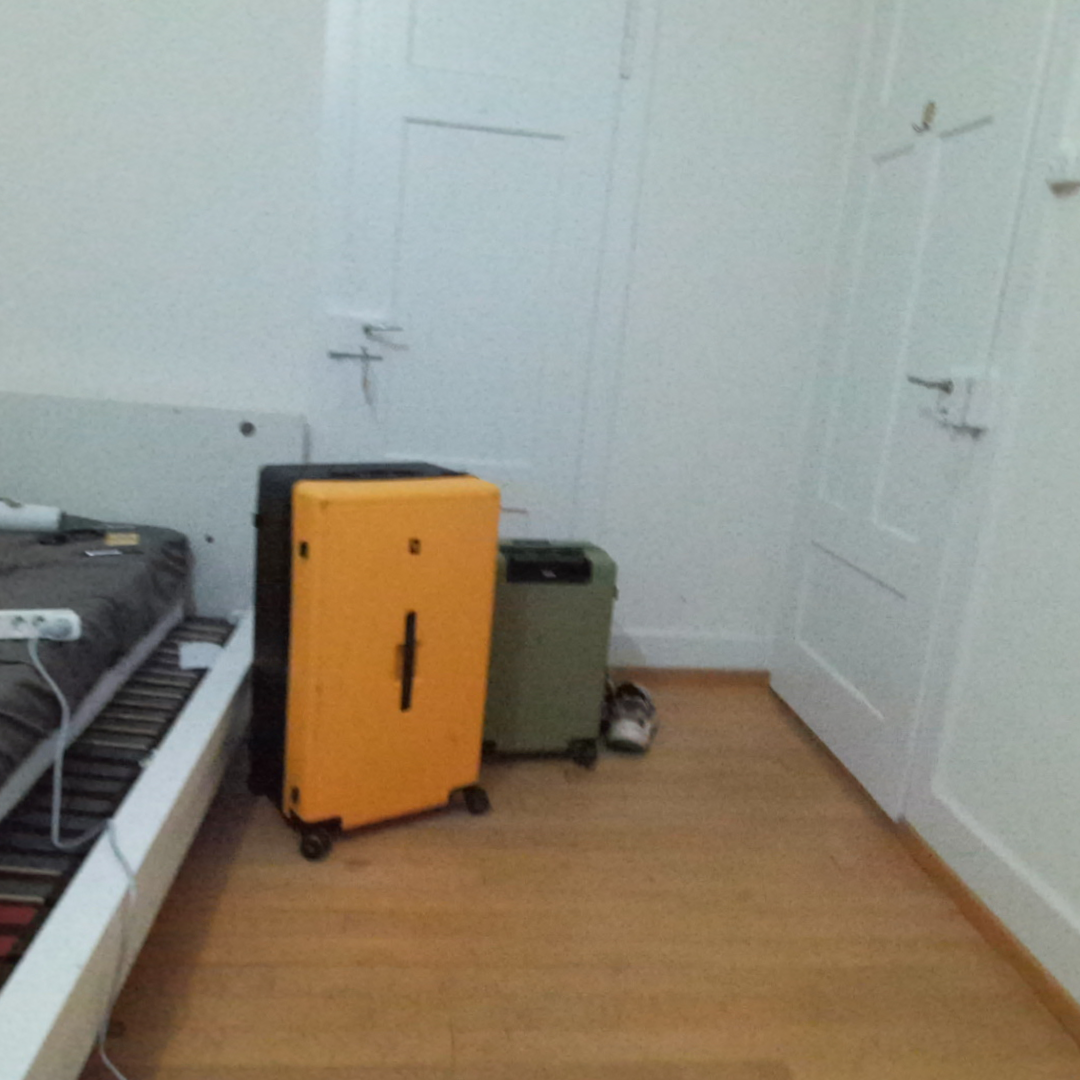
\includegraphics[width=156\unitlength]{figures/export_lossless/real_across_before_9a1e1fb8.png}}%
\dsbox{34.667}{190.478}{58.067}{61.678}%
% real_within_before.png; square source crop [420, 0, 1500, 1080]
\put(160,160){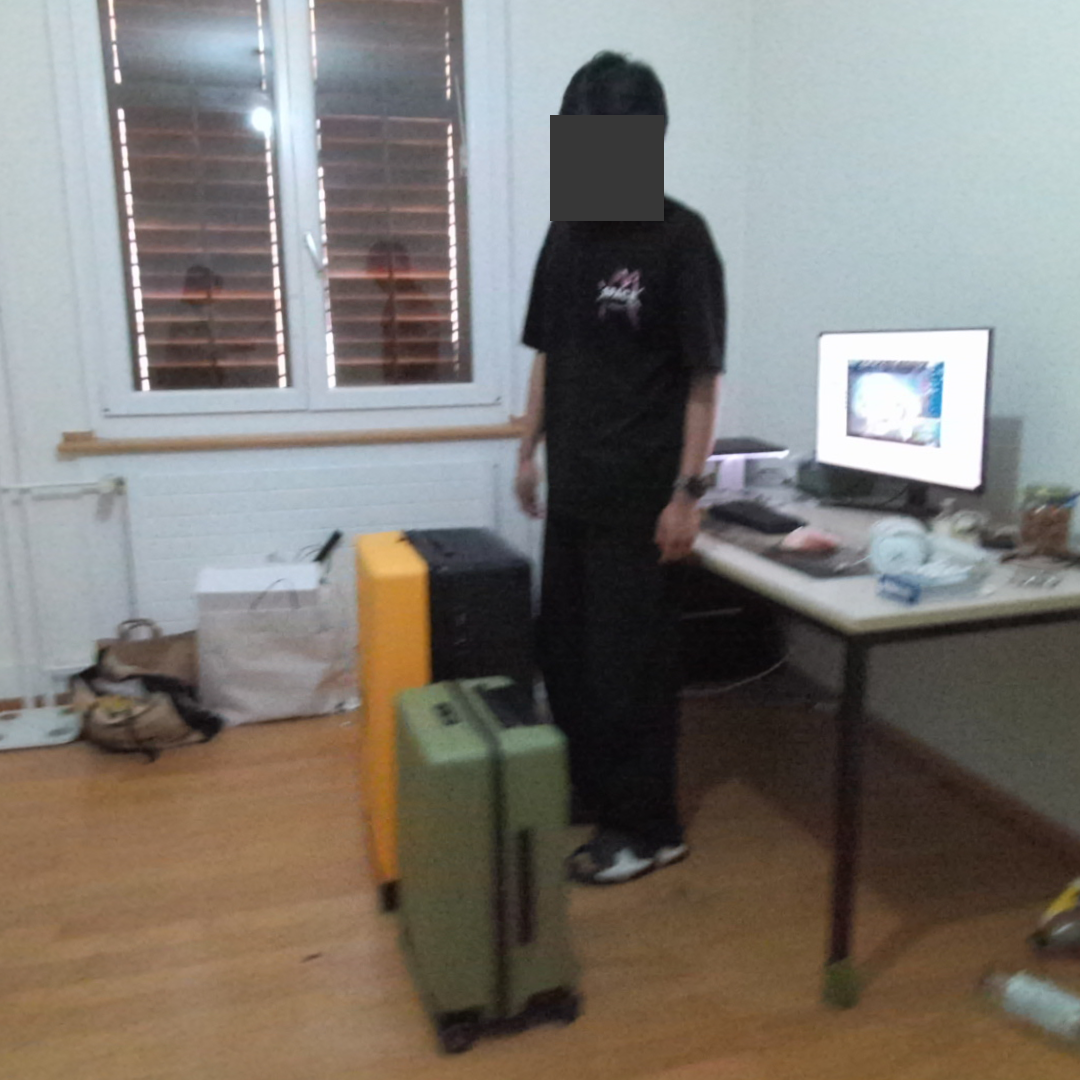
\includegraphics[width=156\unitlength]{figures/privacy/face_redacted_1.png}}%
\dsbox{207.956}{161.300}{38.567}{81.033}%
% real_within_after.png; square source crop [420, 0, 1500, 1080]
\put(320,160){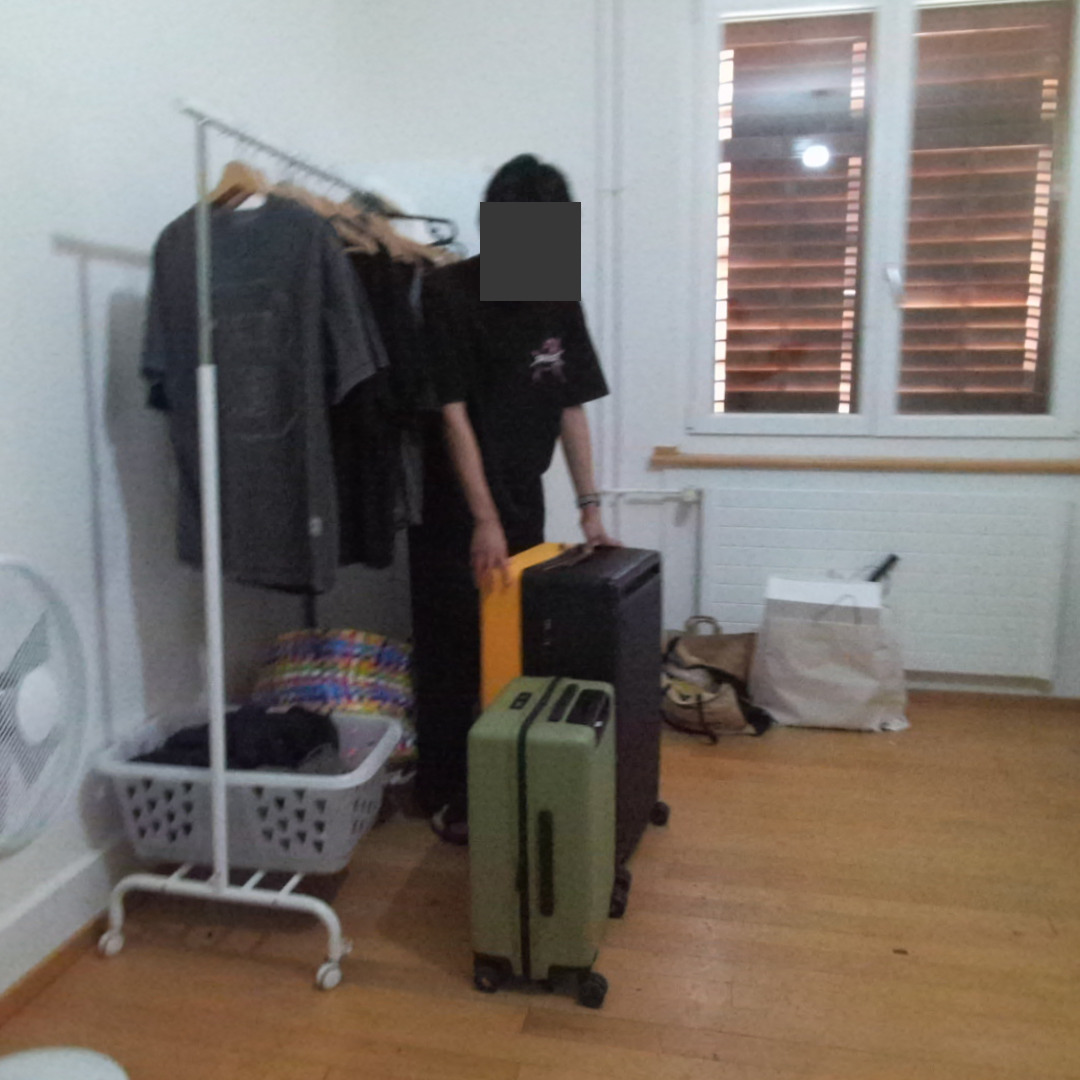
\includegraphics[width=156\unitlength]{figures/privacy/face_redacted_2.png}}%
\dsbox{384.711}{170.400}{34.089}{69.333}%
% sim_furniture_previous.png; square source crop [200, 0, 1000, 800]
\put(0,0){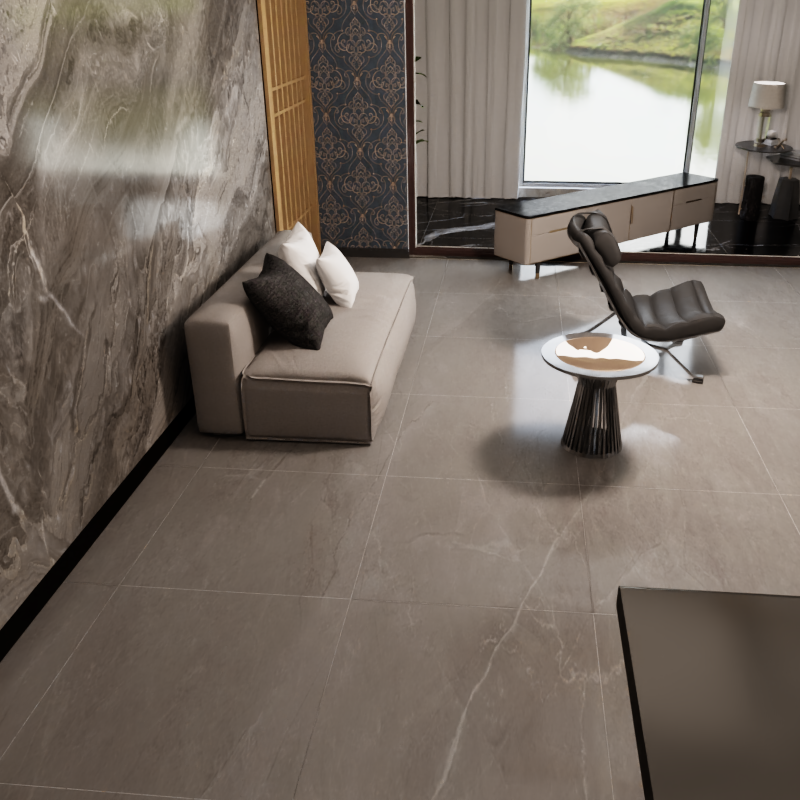
\includegraphics[width=156\unitlength]{figures/export_lossless/sim_furniture_previous_758651d2.png}}%
\dsbox{32.955}{66.690}{50.700}{46.995}%
% sim_furniture_before.png; square source crop [430, 0, 1230, 800]
\put(160,0){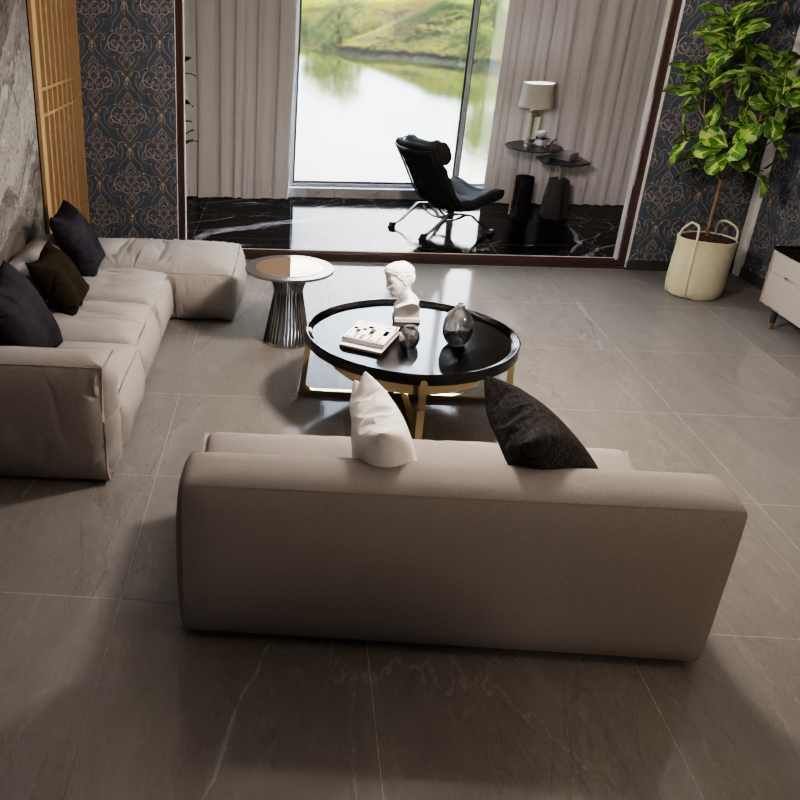
\includegraphics[width=156\unitlength]{figures/export_lossless/sim_furniture_before_28b28c6d.png}}%
\dsbox{191.590}{22.620}{118.755}{64.545}%
% sim_furniture_after.png; square source crop [20, 0, 820, 800]
\put(320,0){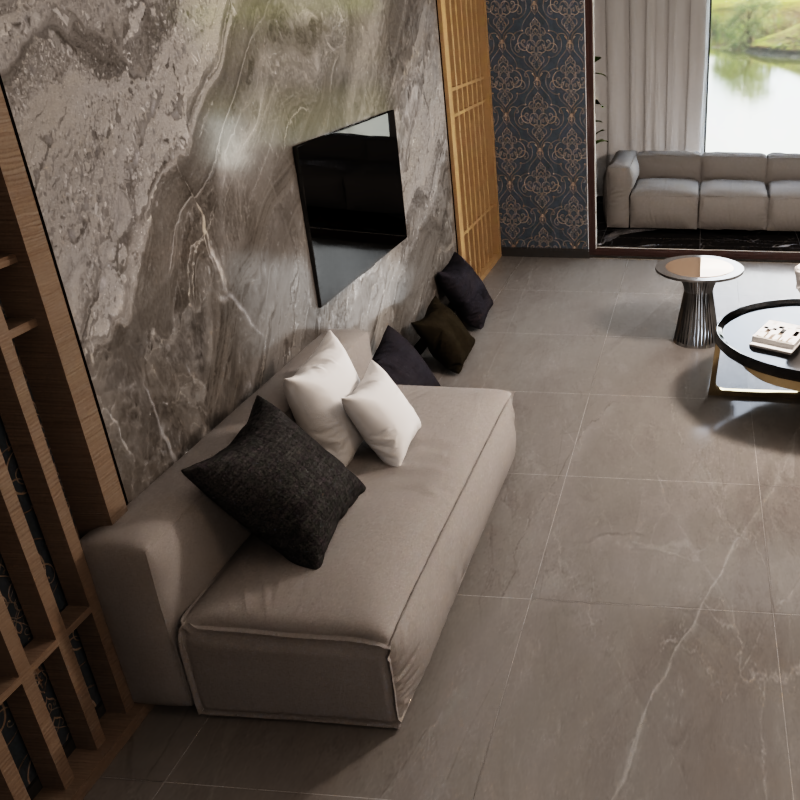
\includegraphics[width=156\unitlength]{figures/export_lossless/sim_furniture_after_09e4278e.png}}%
\dsbox{329.360}{10.530}{95.160}{84.435}%
\end{picture}%
\endgroup
\caption{\textbf{Scene changes across and within visits.}
Each sequence shows the previous visit and a change during the current visit.
Boxes follow the suitcases in the real room (top) and the sofa in the simulated apartment (bottom).}
\label{fig:dataset_changes}
\end{figure}
% ===== END figures / dataset_overview_main =====



\noindent\textbf{Real-world recordings.}
We recorded three visits to the same room over two weeks
using an Azure Kinect. Objects move within visits and are rearranged
between visits, while moving people, depth noise, and partial views
introduce the challenges of real-world mapping.
Camera poses are estimated with ORB-SLAM3~\cite{9440682}. We annotate object identities and changes over time,
yielding 31 reference change events across the three visits (5 within visits and 26 between visits),
and provide a reference reconstruction for geometric evaluation.

\noindent\textbf{Simulated sequences.}
We rendered two animated visits to an InteriorAgent
apartment~\cite{InteriorAgent2025} in Isaac Sim, with object changes
within and between visits. The simulator provides ground-truth
camera poses, object labels, and scene geometry over time.
The second visit covers only part of the apartment, which tests
whether a continued map keeps what the revisit does not see.
The two visits contain 72 reference change events (38 within visits and 34 between visits).



\section{Experiments}
\label{sec:experiments}

We evaluate map accuracy across representations, reconstruction of changes over time,
and Gaussian novel-view quality. Ablations examine the contributions of geometry
retirement and observation validity.
% Keep the expanded result figures close to their corresponding analyses.
\setlength{\textfloatsep}{12pt plus 2pt minus 2pt}
\setlength{\dbltextfloatsep}{12pt plus 2pt minus 2pt}
\setlength{\floatsep}{8pt plus 2pt minus 2pt}
\setlength{\dblfloatsep}{8pt plus 2pt minus 2pt}

% ===== BEGIN tables / main_results =====
% Values: wt_takeover_runs/RESULTS_TABLE_20261029.md (main table, 11-04).
\begin{table*}[t]
\centering
\small
\setlength{\tabcolsep}{3pt}
\renewcommand{\arraystretch}{1.15}
\def\resultrows{
\toprule
& & \multicolumn{6}{c}{\textbf{Within and across visits}} & \multicolumn{6}{c}{\textbf{Across visits}} \\
\cmidrule(lr){3-8}\cmidrule(lr){9-14}
& & \multicolumn{3}{c}{Real} & \multicolumn{3}{c}{Sim} & \multicolumn{3}{c}{Flat} & \multicolumn{3}{c}{3RScan} \\
\cmidrule(lr){3-5}\cmidrule(lr){6-8}\cmidrule(lr){9-11}\cmidrule(lr){12-14}
Map & Method & Mesh & Obj. & Chg. & Mesh & Obj. & Chg. & Mesh & Obj. & Chg. & Mesh & Obj. & Chg. \\
\midrule
 & Khronos~\cite{Schmid-RSS-24} & 87.7 & 78.5 & 70.8 & 93.1 & 80.2 & 84.0 & 86.9 & 45.4 & 53.3 & 88.8 & 65.6 & 73.3 \\
 & Panoptic~\cite{9811877} & 87.3 & 63.4 & 50.0 & 92.4 & 76.6 & 73.5 & 89.4 & 45.3 & 55.6 & 81.0 & 54.9 & 44.6 \\
\multirow{-3}{*}{TSDF} & \oursname & \ob{96.1} & \ob{96.6} & \ob{98.4} & \ob{99.2} & \ob{83.6} & \ob{97.9} & \ob{90.1} & \ob{50.7} & \ob{76.5} & \ob{91.8} & \ob{68.6} & \ob{80.5} \\
\midrule
 & GaME~\cite{Yugay_2026_CVPR} & 88.6 & 76.9 & 96.7 & 80.9 & 72.6 & 82.9 & 86.2 & 65.2 & 76.5 & 85.9 & 77.5 & 87.8 \\
\multirow{-2}{*}{3DGS} & \oursname & \ob{95.1} & \ob{94.0} & \ob{98.4} & \ob{96.5} & \ob{84.0} & \ob{97.9} & \ob{89.0} & \ob{67.1} & \ob{83.3} & \ob{89.6} & \ob{82.6} & \ob{96.1} \\
\midrule
 & Wavemap~\cite{Reijgwart-RSS-23} & 84.5 & 80.0 & 89.7 & 93.2 & 82.6 & 96.4 & 80.2 & 54.1 & 92.3 & 75.6 & 79.5 & 95.3 \\
\multirow{-2}{*}{Occupancy} & \oursname & \ob{91.0} & \ob{93.8} & \ob{100.0} & \ob{94.2} & \ob{86.5} & \ob{98.6} & \ob{82.4} & \ob{55.4} & \ob{95.0} & \ob{79.4} & \ob{80.6} & \ob{97.4} \\
\bottomrule
}
\sbox0{\begin{tabular}{llrrr@{\hspace{10pt}}rrr@{\hspace{10pt}}rrr@{\hspace{10pt}}rrr}\resultrows\end{tabular}}
\setlength{\tabcolsep}{\dimexpr\tabcolsep+(\linewidth-\wd0)/22\relax}
\begin{tabular}{llrrr@{\hspace{10pt}}rrr@{\hspace{10pt}}rrr@{\hspace{10pt}}rrr}\resultrows\end{tabular}
\caption{\textbf{Dynamic mapping within and across visits.} Mesh, object, and change F1 (\%, higher is better);
mesh F1 uses a 5\,cm threshold. Within each map representation, bold marks the best score and shading marks our
rows.}
\label{tab:main}
\end{table*}
% ===== END tables / main_results =====

\noindent\textbf{Datasets.}
Besides DynaState (\cref{sec:benchmark}), we evaluate changes across visits on
Flat~\cite{9811877}, a simulated apartment, eight real-world rooms from
3RScan~\cite{9010673}, and Aria recordings~\cite{Yugay_2026_CVPR}.
For changes within a visit, we use Khronos's TESSE Office
and Apartment sequences~\cite{Schmid-RSS-24}.

\noindent\textbf{Baselines and protocol.}
We compare each representation with its native update:
Khronos~\cite{Schmid-RSS-24} and Panoptic Multi-TSDFs~\cite{9811877}
for TSDF, GaME~\cite{Yugay_2026_CVPR} for Gaussians,
and Wavemap~\cite{Reijgwart-RSS-23} for occupancy.
Within each table, methods receive the same posed frames and segmentation inputs.


\noindent\textbf{Metrics.}
We evaluate geometric accuracy and completeness using
mesh F1~\cite{Knapitsch2017} at a 5\,cm threshold.
For Gaussian maps, we extract meshes by TSDF fusion
of rendered depth maps, following 2DGS~\cite{Huang2DGS2024}.
Following Khronos~\cite{Schmid-RSS-24}, we use object F1 to measure
the accuracy and completeness of mapped objects, and change F1
to evaluate the detection of object appearances and disappearances.
Rendering is evaluated on held-out views following GaME~\cite{Yugay_2026_CVPR},
using PSNR, MS-SSIM~\cite{1292216}, LPIPS~\cite{Zhang_2018_CVPR},
and depth L1.
Gaussian geometry and rendering are evaluated after refinement.


\subsection{Dynamic Mapping within and across Visits}
\label{sec:exp_main}


Across all three representations and four datasets, \ours improves mesh, object,
and change F1 over the native updates under the same instance-mask inputs
(\cref{tab:main}). \Cref{fig:geometry_details} shows the reconstructions after scene changes.

% ===== BEGIN figures / qualitative_combined =====
% Two alternatives for Figure 4. Keep exactly one option uncommented.
% To switch: comment the active option and uncomment the other with Ctrl+/.
% ===== OPTION A: HORIZONTAL / 5 rows x 6 columns / two-column width =====
\begin{figure*}[!t]
\centering
\begingroup%
\rmfamily\fontsize{8}{9}\selectfont%
\setlength{\unitlength}{\dimexpr\linewidth/629\relax}%
\begin{picture}(629,534)%
\put(64,524){\makebox(0,0){Panoptic~\cite{9811877}}}%
\put(167,524){\makebox(0,0){Khronos~\cite{Schmid-RSS-24}}}%
\put(270,524){\makebox(0,0){Wavemap~\cite{Reijgwart-RSS-23}}}%
\put(373,524){\makebox(0,0){GaME~\cite{Yugay_2026_CVPR}}}%
\put(476,524){\makebox(0,0){\textbf{Ours (3DGS)}}}%
\put(579,524){\makebox(0,0){Ground Truth}}%
\put(4,462){\makebox(0,0){\rotatebox[origin=c]{90}{Real C}}}%
\put(14,412){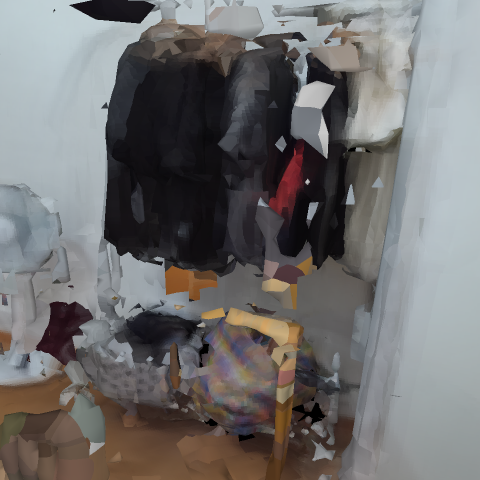
\includegraphics[width=100\unitlength]{figures/export_lossless/2_panoptic_a8edd3e3.png}}%
\put(117,412){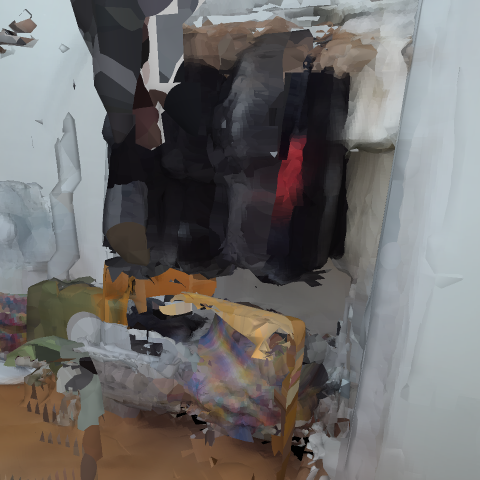
\includegraphics[width=100\unitlength]{figures/export_lossless/1_khronos_a9f68713.png}}%
\put(220,412){\includegraphics[width=100\unitlength]{figures/export_lossless/6_Wavemap_ac73dda5.png}}%
\put(323,412){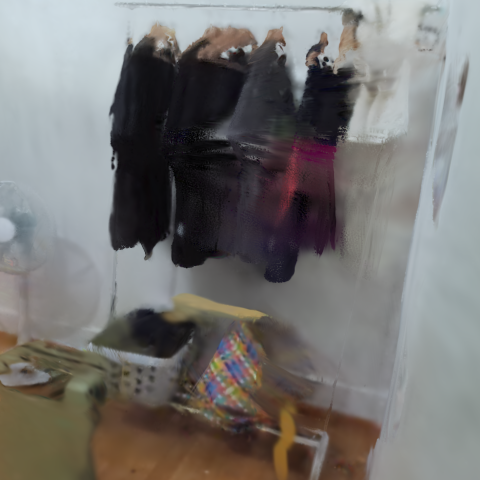
\includegraphics[width=100\unitlength]{figures/export_lossless/4_game_519ea7a8.png}}%
\put(426,412){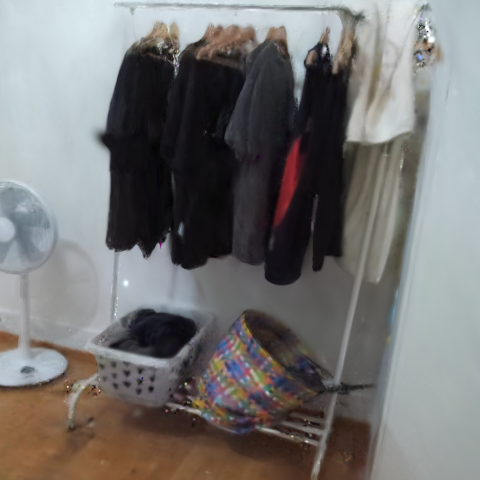
\includegraphics[width=100\unitlength]{figures/export_lossless/5_ours_3dgs_3e673e58.png}}%
\put(529,412){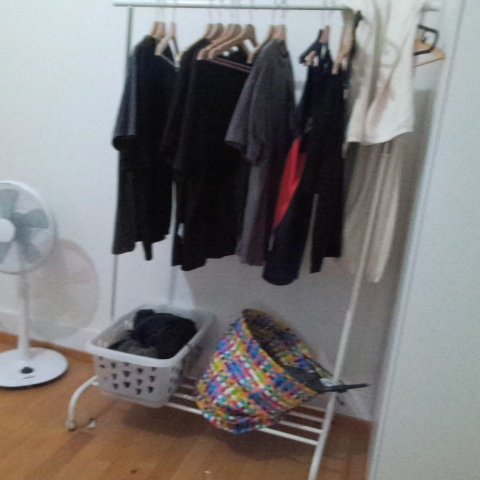
\includegraphics[width=100\unitlength]{figures/export_lossless/0_image_b5dac36e.png}}%
\put(4,359){\makebox(0,0){\rotatebox[origin=c]{90}{Real C}}}%
\put(14,309){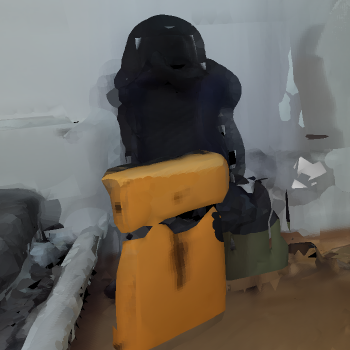
\includegraphics[width=100\unitlength]{figures/export_lossless/2_panoptic_70c53c8a.png}}%
\put(117,309){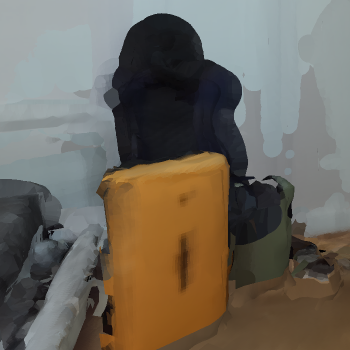
\includegraphics[width=100\unitlength]{figures/export_lossless/1_khronos_6aa9b730.png}}%
\put(220,309){\includegraphics[width=100\unitlength]{figures/export_lossless/6_Wavemap_41c23c24.png}}%
\put(323,309){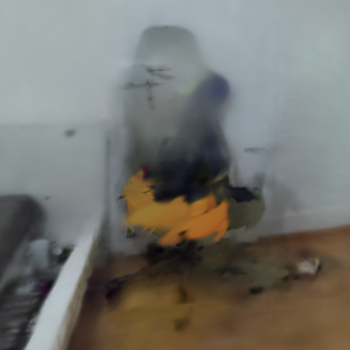
\includegraphics[width=100\unitlength]{figures/export_lossless/4_game_227900b4.png}}%
\put(426,309){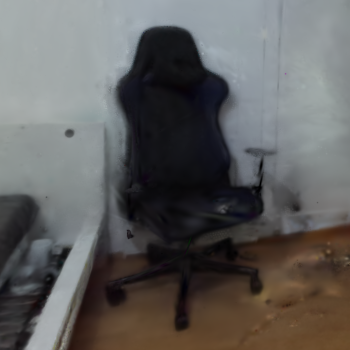
\includegraphics[width=100\unitlength]{figures/export_lossless/5_ours_3dgs_0081864f.png}}%
\put(529,309){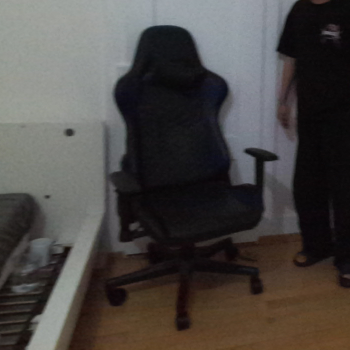
\includegraphics[width=100\unitlength]{figures/export_lossless/0_image_1983d228.png}}%
\put(4,256){\makebox(0,0){\rotatebox[origin=c]{90}{Sim B}}}%
\put(14,206){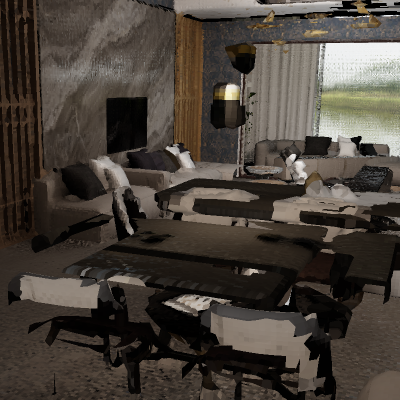
\includegraphics[width=100\unitlength]{figures/export_lossless/2_panoptic_0c07267f.png}}%
\put(117,206){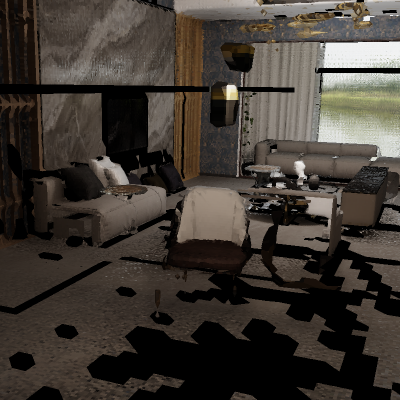
\includegraphics[width=100\unitlength]{figures/export_lossless/1_khronos_285f7d36.png}}%
\put(220,206){\includegraphics[width=100\unitlength]{figures/export_lossless/6_Wavemap_32bae90a.png}}%
\put(323,206){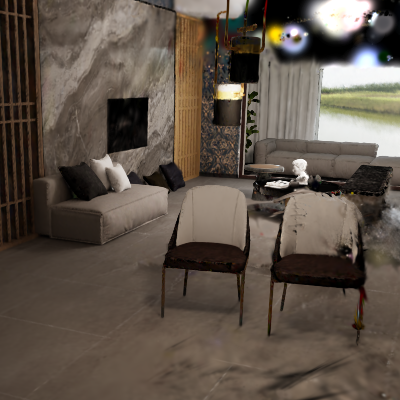
\includegraphics[width=100\unitlength]{figures/export_lossless/4_game_5ac6469c.png}}%
\put(426,206){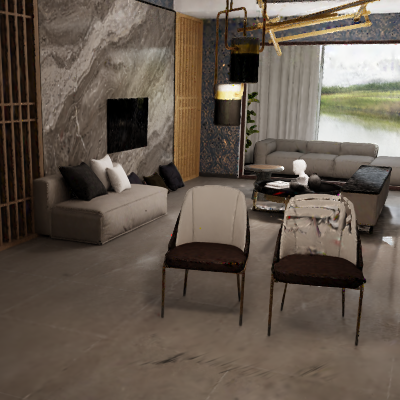
\includegraphics[width=100\unitlength]{figures/export_lossless/5_ours_3dgs_051deed0.png}}%
\put(529,206){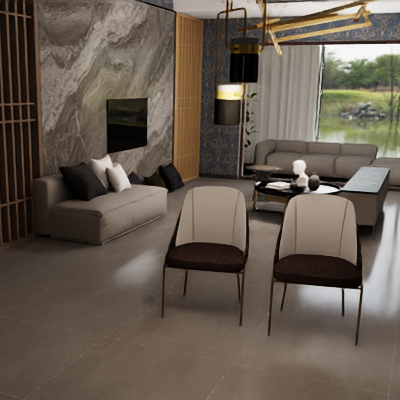
\includegraphics[width=100\unitlength]{figures/export_lossless/0_image_4a8dffdc.png}}%
\put(4,153){\makebox(0,0){\rotatebox[origin=c]{90}{Sim B}}}%
\put(14,103){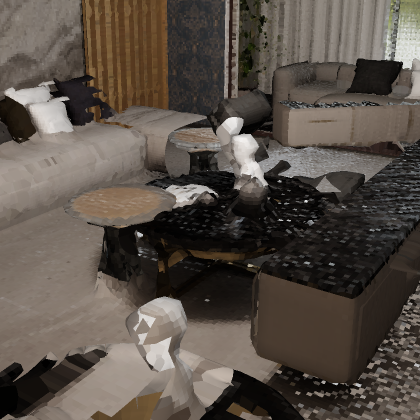
\includegraphics[width=100\unitlength]{figures/export_lossless/2_panoptic_9914928d.png}}%
\put(117,103){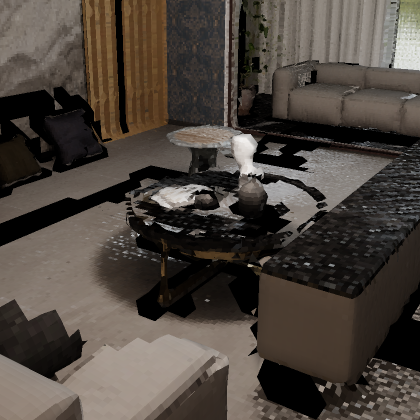
\includegraphics[width=100\unitlength]{figures/export_lossless/1_khronos_008ec86c.png}}%
\put(220,103){\includegraphics[width=100\unitlength]{figures/export_lossless/6_Wavemap_98d063c5.png}}%
\put(323,103){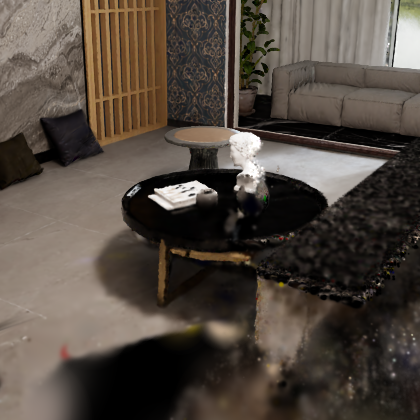
\includegraphics[width=100\unitlength]{figures/export_lossless/4_game_deced8d4.png}}%
\put(426,103){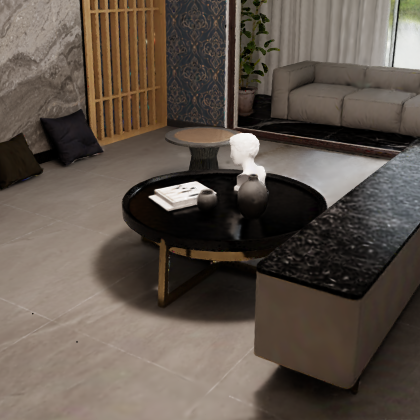
\includegraphics[width=100\unitlength]{figures/export_lossless/5_ours_3dgs_8ed4723d.png}}%
\put(529,103){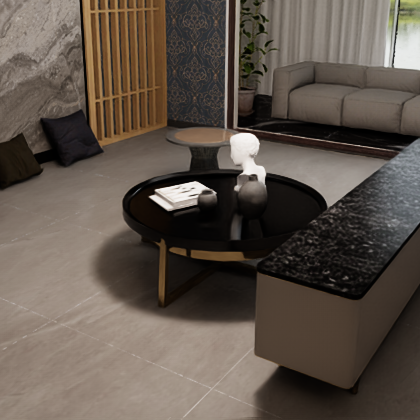
\includegraphics[width=100\unitlength]{figures/export_lossless/0_image_82504eaf.png}}%
\put(4,50){\makebox(0,0){\rotatebox[origin=c]{90}{Flat B}}}%
\put(14,0){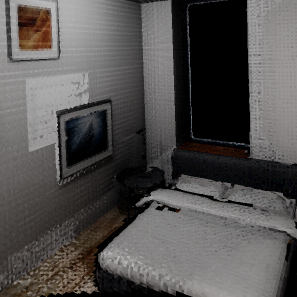
\includegraphics[width=100\unitlength]{figures/export_lossless/2_panoptic_2bf4a7ac.png}}%
\put(117,0){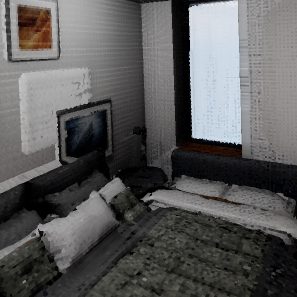
\includegraphics[width=100\unitlength]{figures/export_lossless/1_khronos_2eb98554.png}}%
\put(220,0){\includegraphics[width=100\unitlength]{figures/export_lossless/6_Wavemap_f2d21301.png}}%
\put(323,0){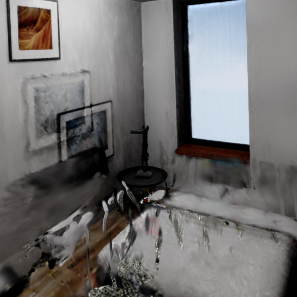
\includegraphics[width=100\unitlength]{figures/export_lossless/4_game_ba3706c3.png}}%
\put(426,0){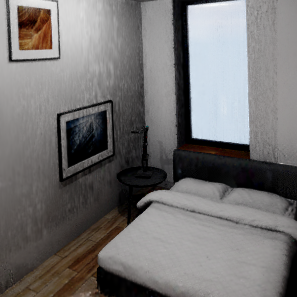
\includegraphics[width=100\unitlength]{figures/export_lossless/5_ours_3dgs_sam_final_7afc0d8c.png}}%
\put(529,0){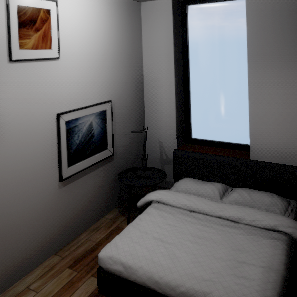
\includegraphics[width=100\unitlength]{figures/export_lossless/0_image_7d65e6a8.png}}%
\end{picture}%
\endgroup%

\caption{\textbf{Reconstructing scenes after changes.} Panoptic, Khronos, Wavemap, GaME, and our Gaussian maps are shown from the same viewpoint alongside the ground-truth image.}
\label{fig:geometry_details}
\label{fig:gaussian_details}
\end{figure*}
% ===== END OPTION A =====

% ===== OPTION B: VERTICAL / 5 rows x 4 columns / single-column width =====
% \begin{figure}[!t]
% \centering
% \begingroup%
% \rmfamily\fontsize{7}{8}\selectfont%
% \setlength{\unitlength}{\dimexpr\linewidth/412\relax}%
% \begin{picture}(412,600)%
% \put(50,590){\makebox(0,0){GT Before (Real)}}%
% \put(154,590){\makebox(0,0){Khronos~\cite{Schmid-RSS-24}}}%
% \put(258,590){\makebox(0,0){Ours (TSDF)}}%
% \put(362,590){\makebox(0,0){GT After (Real)}}%
% \put(0,480){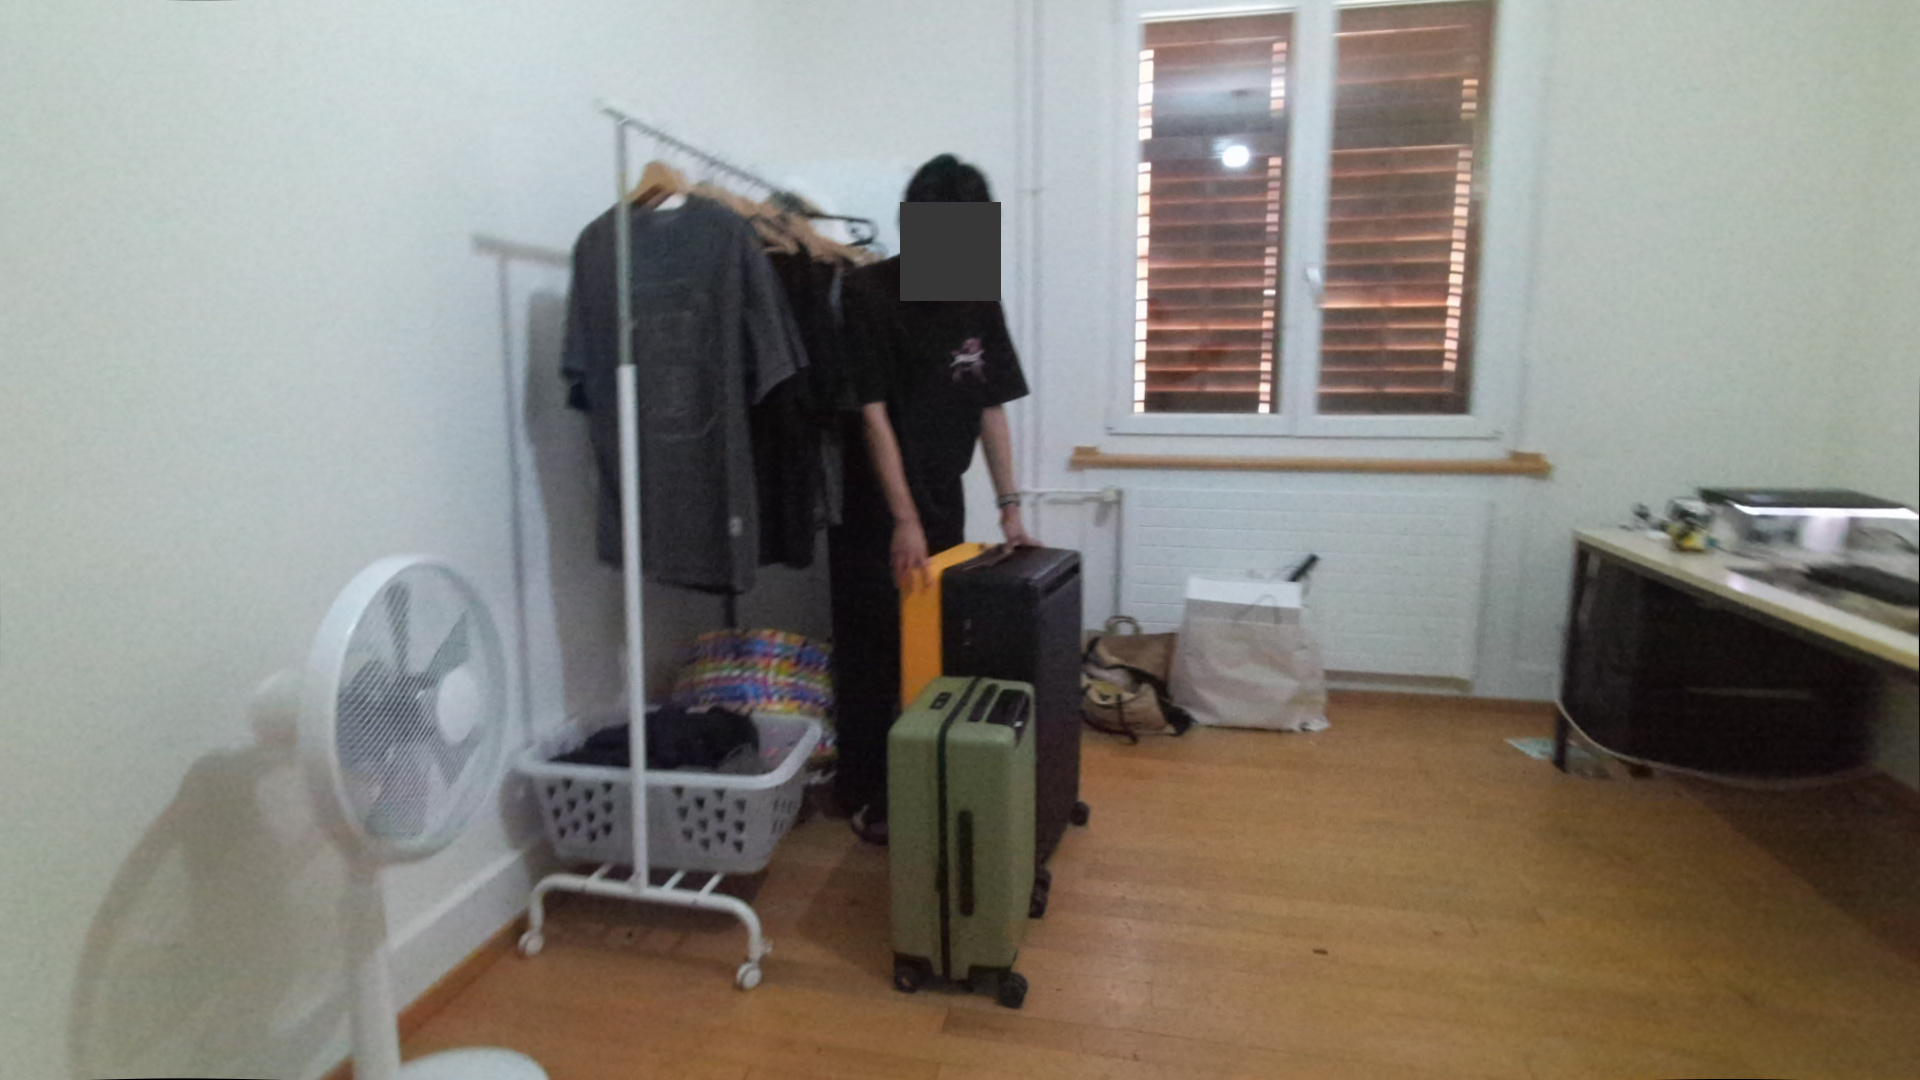
\includegraphics[width=100\unitlength,trim={650bp 50bp 620bp 380bp},clip]{figures/privacy/face_redacted_4.png}}%
% \put(104,480){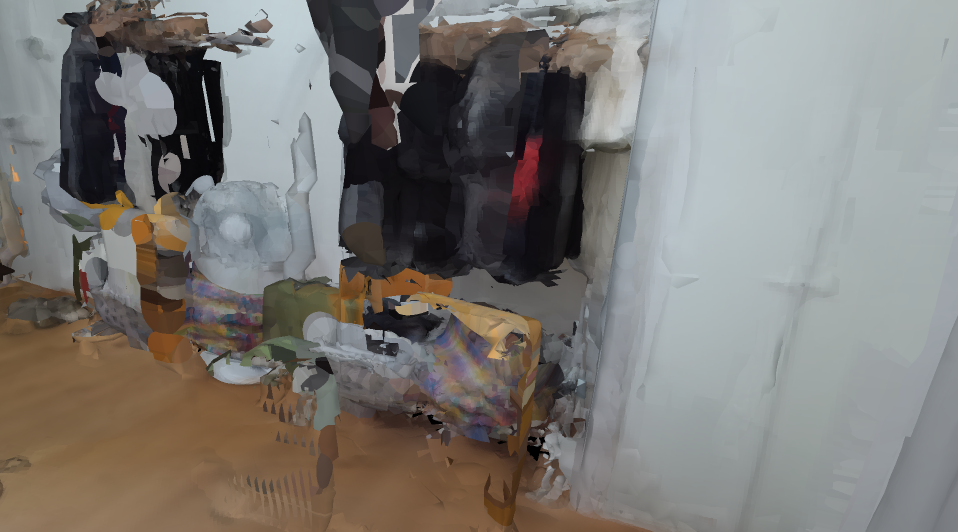
\includegraphics[width=100\unitlength,trim={210bp 0bp 216bp 0bp},clip]{figures/results_native/qual/1_real_05320/1_khronos.png}}%
% \put(208,480){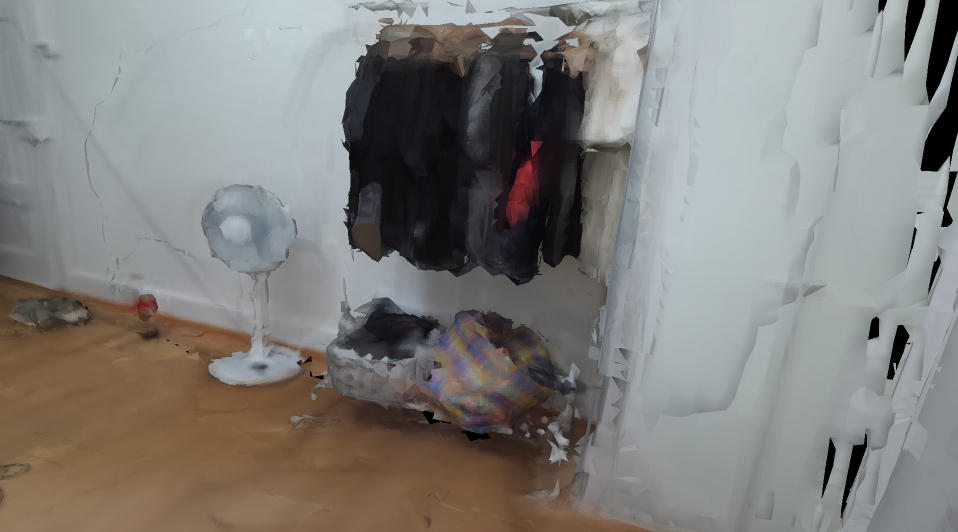
\includegraphics[width=100\unitlength,trim={210bp 0bp 216bp 0bp},clip]{figures/results_native/qual/1_real_05320/3_ours_tsdf.png}}%
% \put(312,480){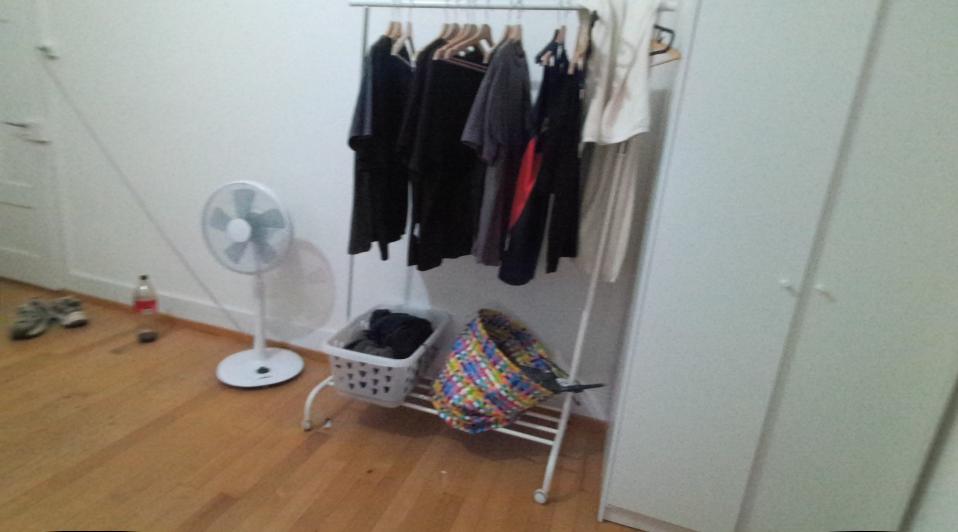
\includegraphics[width=100\unitlength,trim={210bp 0bp 216bp 0bp},clip]{figures/results_native/qual/1_real_05320/0_image.png}}%
% \put(50,470){\makebox(0,0){GT Before (Sim)}}%
% \put(154,470){\makebox(0,0){Panoptic~\cite{9811877}}}%
% \put(258,470){\makebox(0,0){Ours (TSDF)}}%
% \put(362,470){\makebox(0,0){GT After (Sim)}}%
% \put(0,360){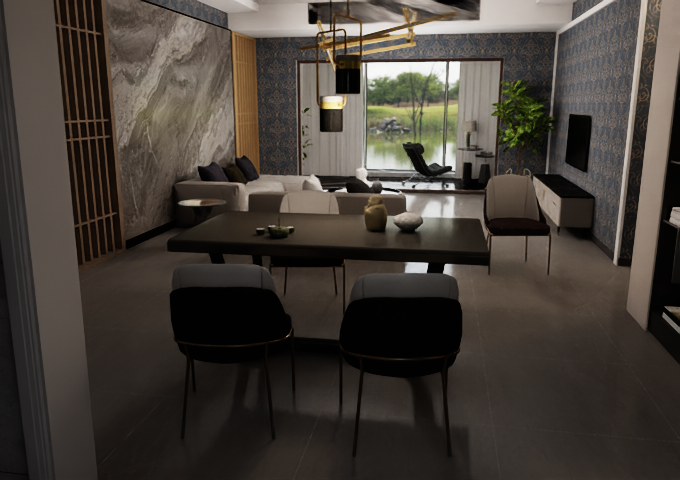
\includegraphics[width=100\unitlength,trim={150bp 35bp 100bp 15bp},clip]{figures/results_native/qual_compact/panoptic_sim_before.png}}%
% \put(104,360){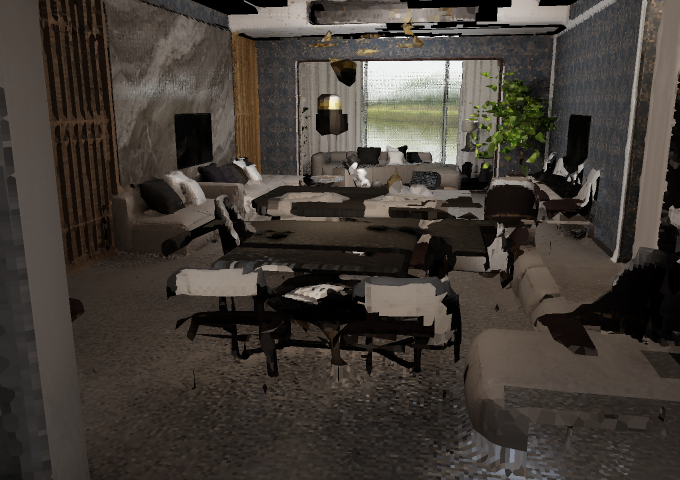
\includegraphics[width=100\unitlength,trim={150bp 35bp 100bp 15bp},clip]{figures/results_native/qual/3_sim_02850/2_panoptic.png}}%
% \put(208,360){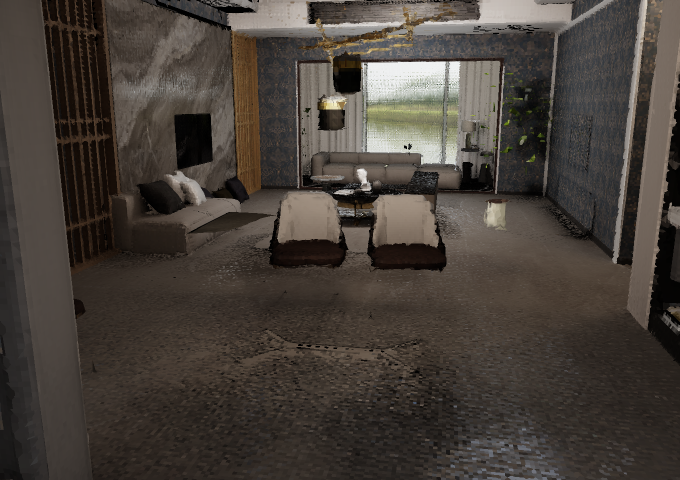
\includegraphics[width=100\unitlength,trim={150bp 35bp 100bp 15bp},clip]{figures/results_native/qual/3_sim_02850/3_ours_tsdf.png}}%
% \put(312,360){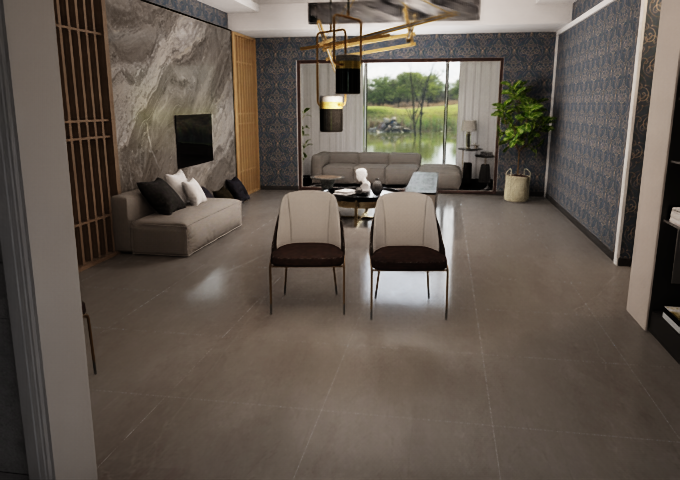
\includegraphics[width=100\unitlength,trim={150bp 35bp 100bp 15bp},clip]{figures/results_native/qual_compact/panoptic_sim_after.png}}%
% \put(50,350){\makebox(0,0){GT Before (Real)}}%
% \put(154,350){\makebox(0,0){Wavemap~\cite{Reijgwart-RSS-23}}}%
% \put(258,350){\makebox(0,0){Ours (Occupancy)}}%
% \put(362,350){\makebox(0,0){GT After (Real)}}%
% \put(0,240){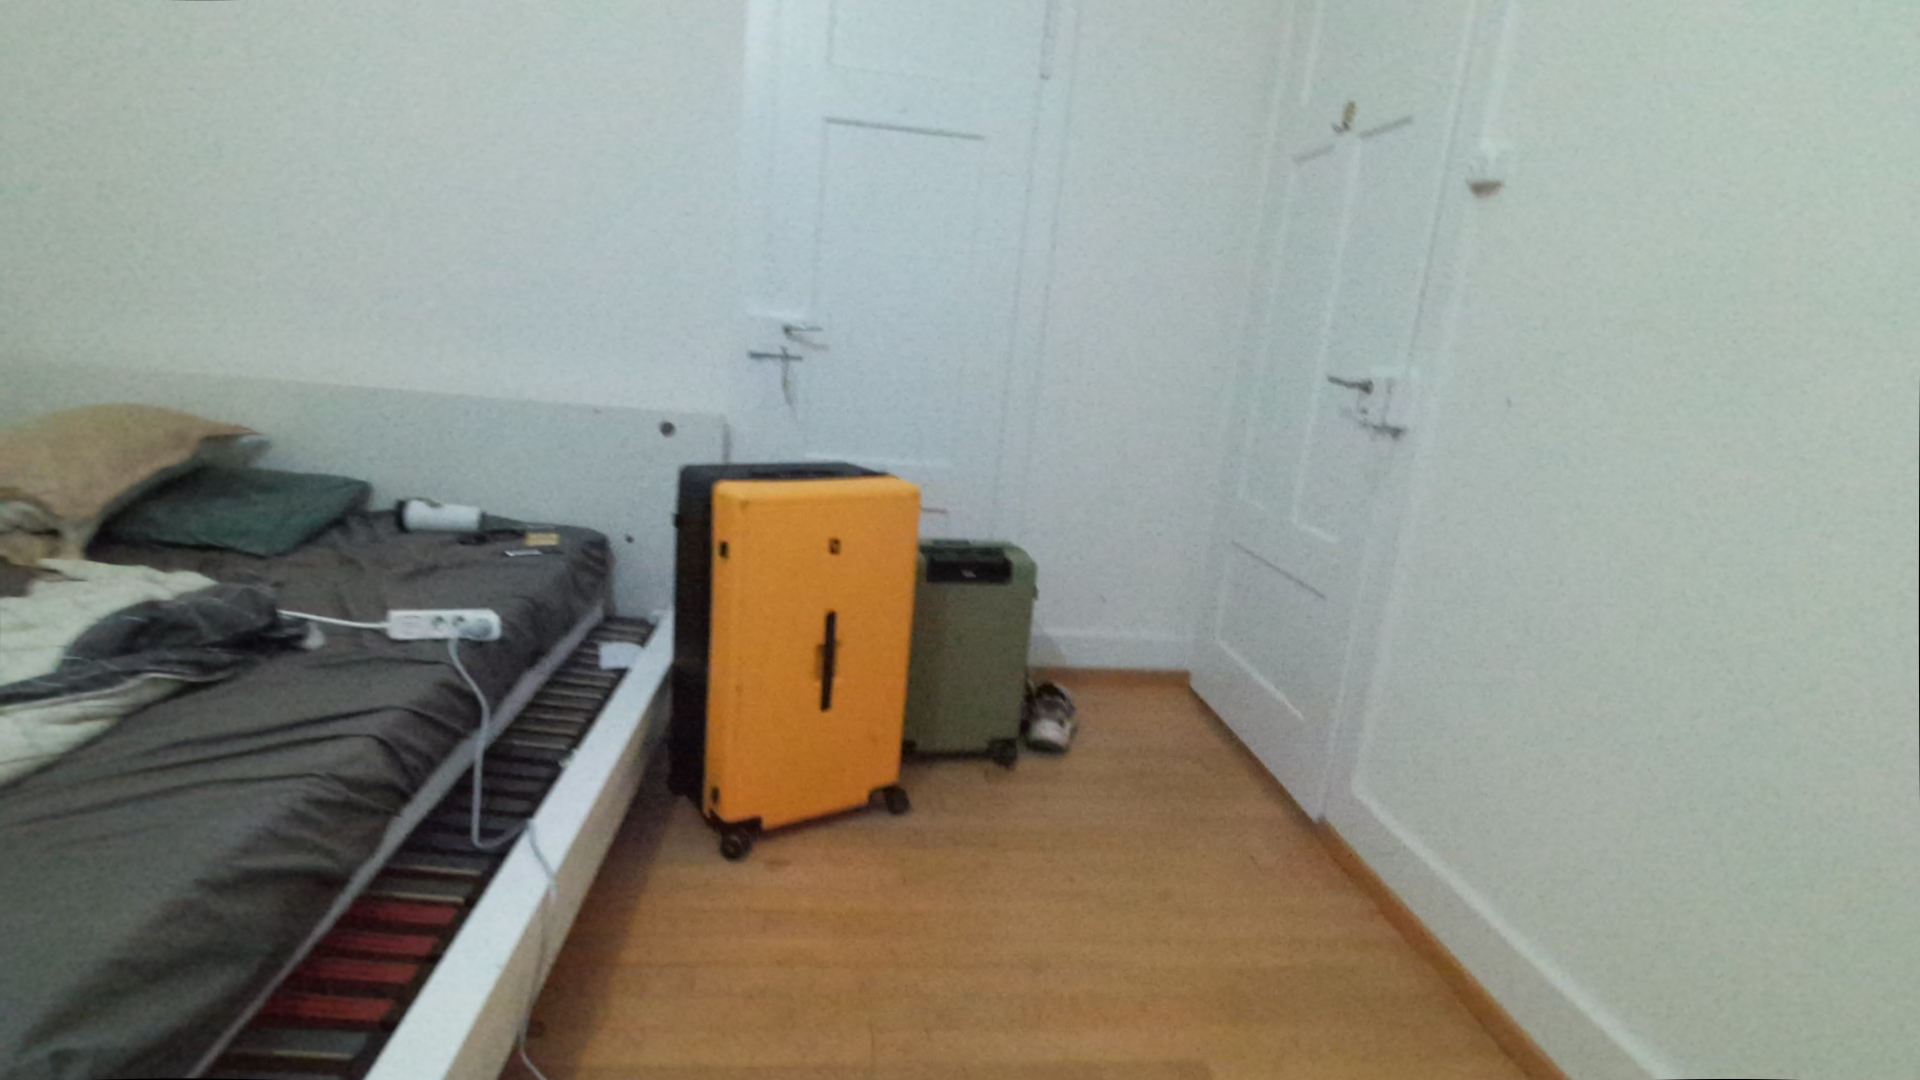
\includegraphics[width=100\unitlength,trim={600bp 80bp 720bp 400bp},clip]{figures/results_native/before_after/real_before_B003120.png}}%
% \put(104,240){\includegraphics[width=100\unitlength,trim={240bp 0bp 336bp 150bp},clip]{figures/results_native/qual_compact/Wavemap_real_02630.png}}%
% \put(208,240){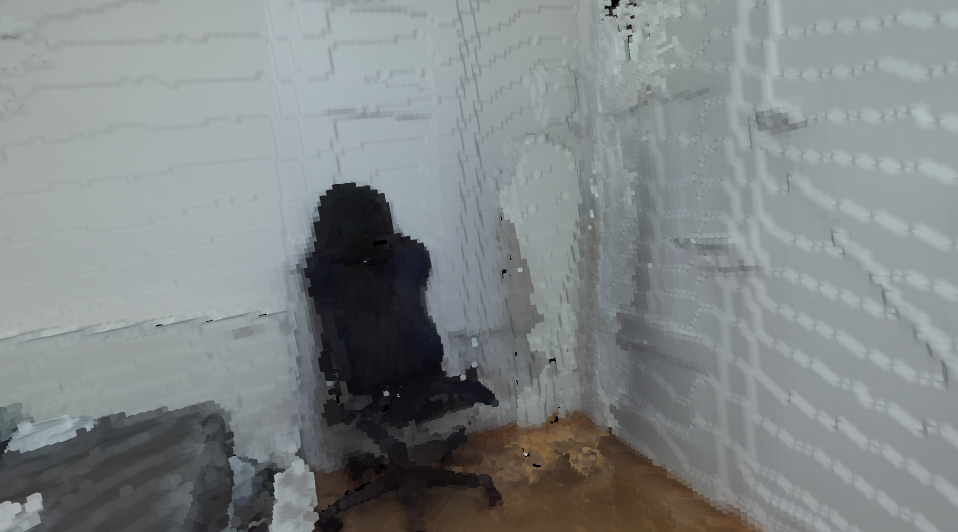
\includegraphics[width=100\unitlength,trim={240bp 0bp 336bp 150bp},clip]{figures/results_native/qual_compact/ours_occ_real_02630.png}}%
% \put(312,240){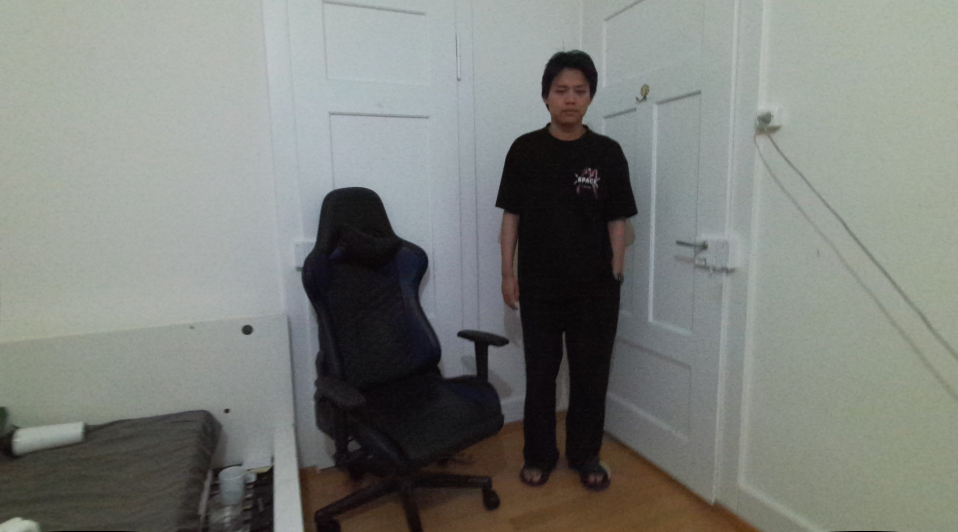
\includegraphics[width=100\unitlength,trim={240bp 0bp 336bp 150bp},clip]{figures/results_native/qual_compact/real_C02630_rgb.png}}%
% \put(50,230){\makebox(0,0){GT Before (Sim)}}%
% \put(154,230){\makebox(0,0){GaME~\cite{Yugay_2026_CVPR}}}%
% \put(258,230){\makebox(0,0){Ours (3DGS)}}%
% \put(362,230){\makebox(0,0){GT After (Sim)}}%
% \put(0,120){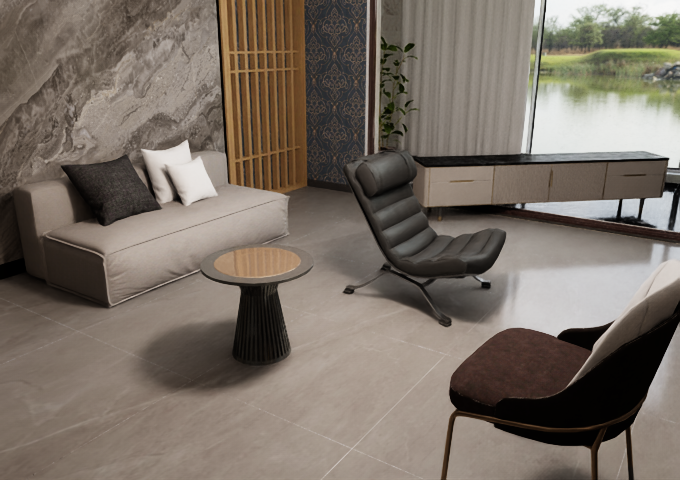
\includegraphics[width=100\unitlength,trim={140bp 0bp 120bp 60bp},clip]{figures/results_native/qual_compact/gaussian_sim_before.png}}%
% \put(104,120){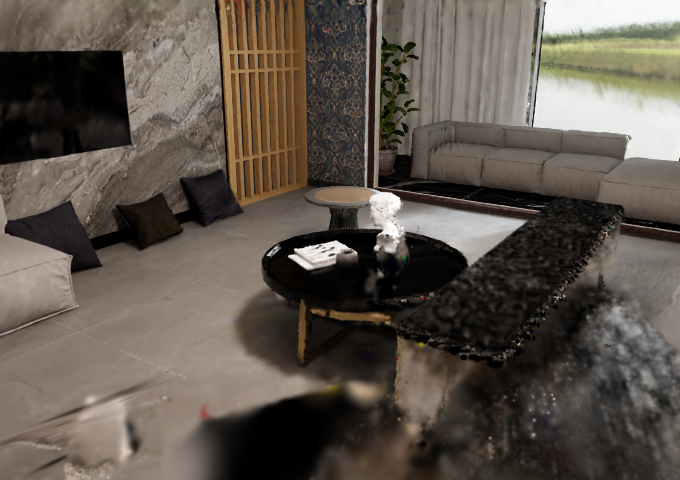
\includegraphics[width=100\unitlength,trim={140bp 0bp 120bp 60bp},clip]{figures/results_native/qual/4_sim_03065/4_game.png}}%
% \put(208,120){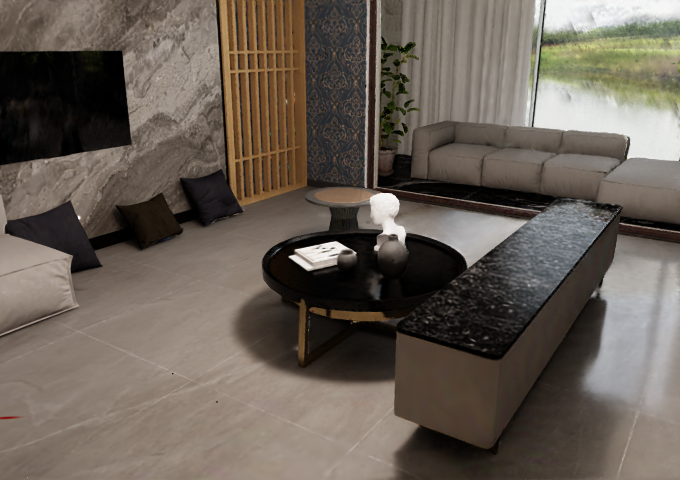
\includegraphics[width=100\unitlength,trim={140bp 0bp 120bp 60bp},clip]{figures/results_native/qual/4_sim_03065/5_ours_3dgs.png}}%
% \put(312,120){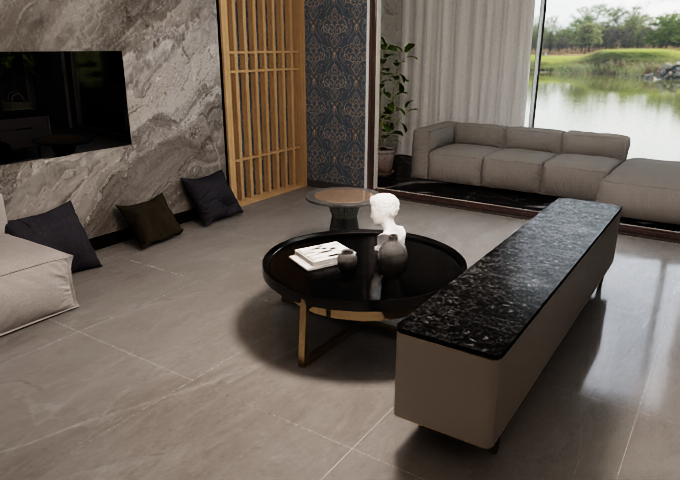
\includegraphics[width=100\unitlength,trim={140bp 0bp 120bp 60bp},clip]{figures/results_native/qual_compact/gaussian_sim_after.png}}%
% \put(50,110){\makebox(0,0){GT Before (Flat)}}%
% \put(154,110){\makebox(0,0){GaME~\cite{Yugay_2026_CVPR}}}%
% \put(258,110){\makebox(0,0){Ours (3DGS)}}%
% \put(362,110){\makebox(0,0){GT After (Flat)}}%
% \put(0,0){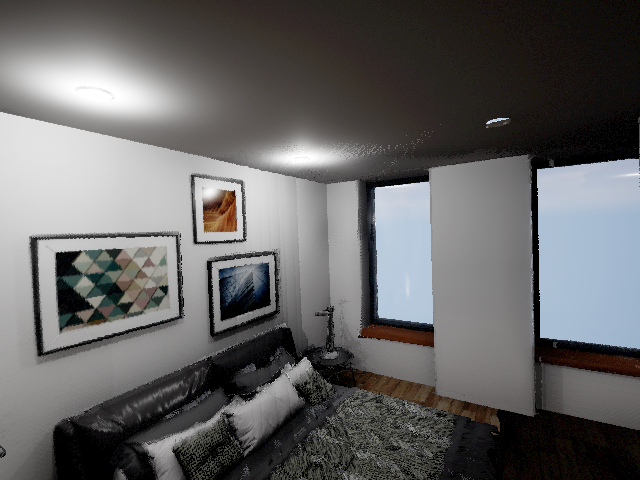
\includegraphics[width=100\unitlength,trim={185bp 2bp 158bp 181bp},clip]{figures/results_native/qual_compact/flat_before_same_view.png}}%
% \put(104,0){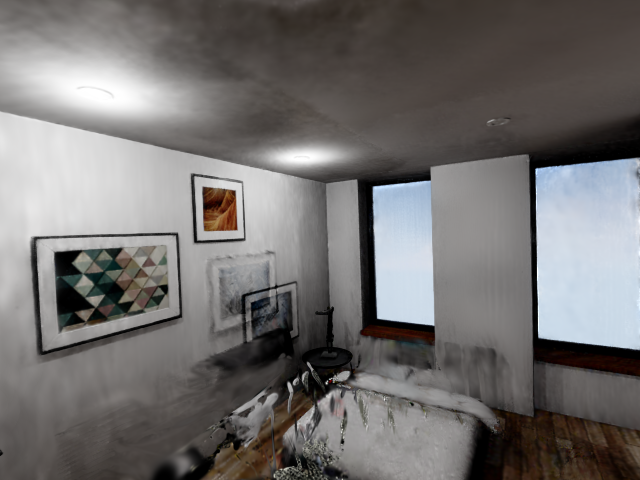
\includegraphics[width=100\unitlength,trim={185bp 2bp 158bp 181bp},clip]{figures/results_native/qual/5_flat_00270/4_game.png}}%
% \put(208,0){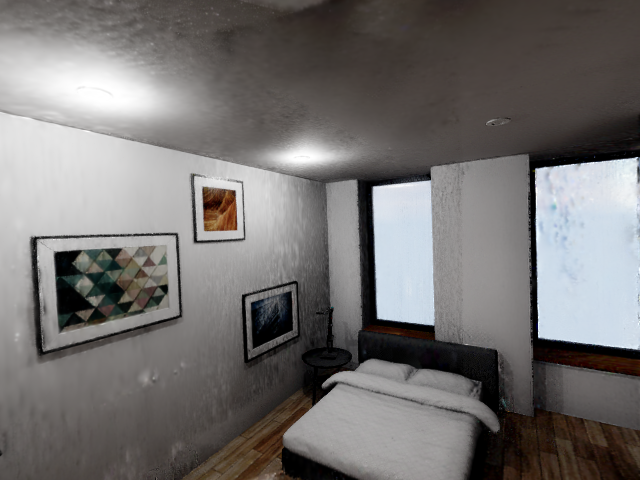
\includegraphics[width=100\unitlength,trim={185bp 2bp 158bp 181bp},clip]{figures/results_native/qual/5_flat_00270/5_ours_3dgs_sam_final.png}}%
% \put(312,0){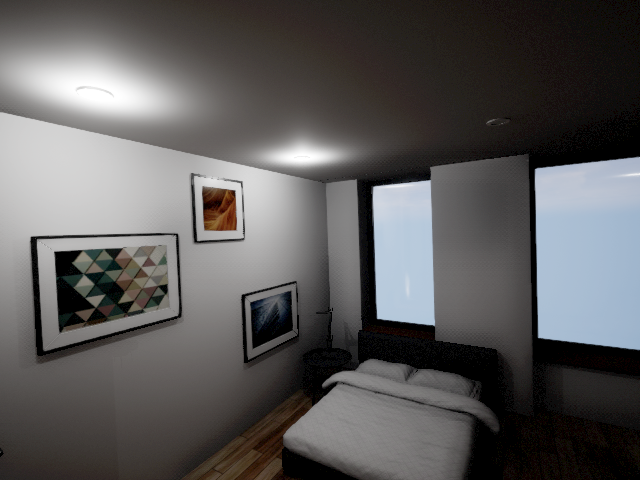
\includegraphics[width=100\unitlength,trim={185bp 2bp 158bp 181bp},clip]{figures/results_native/qual/5_flat_00270/0_image.png}}%
% \end{picture}%
% \endgroup%
%
% \caption{\textbf{Cleaner reconstructions after scene changes.} Before and after views show the scene change. Each baseline and our update use the same representation and viewpoint.}
% \label{fig:geometry_details}
% \label{fig:gaussian_details}
% \end{figure}
% ===== END OPTION B =====
% ===== END figures / qualitative_combined =====

\noindent\textbf{TSDF.}
The gains are largest where the scene changes most. In the real room, mesh F1 rises from 87.7 to 96.1 over
Khronos continuing its map, object F1 from 78.5 to 96.6, and change F1 from 70.8 to 98.4. Khronos verifies absence using rays between reconstructed background
vertices and camera poses. We assess absence from new depth images
at the object's own surface and apply a confirmed change to its
full geometry. The valid domains also stop earlier free space at
new objects, so old observations do not carve away newly added geometry, which raises precision and recall together. Panoptic Multi-TSDFs compares whole submaps against
the active ones and marks a submap absent when enough of its points conflict.
On 3RScan, its change F1 is 44.6, while ours reaches 80.5. Continuing the map also pays off when a revisit
covers only part of the scene: on Sim visit~B, our continued TSDF map reaches 99.2 mesh F1, 9.3 points above a
restart of our mapper and 12.6 above a restart of Khronos (see supplement).

\noindent\textbf{3D Gaussians.}
Our Gaussian maps exceed GaME in mesh F1 by 6.5 points in the real room and 15.6 in the synthetic apartment, in
object F1 by 17.1 and 11.4, and in change F1 by 1.7 and 15.0.
GaME propagates local rendering conflicts through historical object masks to remove stale geometry.
Our state decisions apply jointly to geometry and observation validity;
the resulting maps have fewer residual surfaces in the illustrated scene changes
(\cref{fig:gaussian_details}). The gains on Flat and
3RScan are smaller, 2.8 and 3.7 mesh F1, but consistent across all three scores. Rendering also improves on these instance-input runs.
On Real, Sim, Flat, and 3RScan, PSNR increases by
1.68, 3.05, 3.43, and 0.96\,dB, respectively.
The corresponding MS-SSIM gains are 0.053, 0.067, 0.030, and 0.035.
LPIPS decreases by 0.084, 0.098, 0.047, and 0.035,
and depth L1 decreases by 1.07, 8.62, 0.60, and 2.16\,cm.

\noindent\textbf{Occupancy.}
Occupancy gains are largest in the real room, with mesh F1 from 84.5 to 91.0 and object F1 from 80.0 to 93.8, and
smallest on the synthetic scenes, within 2.2 mesh F1 on Sim and Flat.
Wavemap's clamped log-odds overwrite a changed cell when new measurements contradict it.
Its measurement model also assigns occupancy to a band behind each measured surface.
Across visits, old occupied layers can remain behind newly observed surfaces,
where free-space updates cannot reach them. Our state-level decisions retire
removed objects, and the surface replacement rule removes these stale copies.




\subsection{Changes within a Single Run and 4D on TESSE}
\label{sec:exp_temporal}

Khronos's TESSE sequences contain observed motion and changes after looking away within one continuous run, and
its official evaluator queries the map at earlier times and scores the background, static objects, dynamic
objects, and changes. With the same semantic mask inputs, our TSDF maps improve all four categories on both scenes and reach higher final mesh F1
(\cref{tab:tesse}). The change score moves most: F1 rises from 46.2 to 78.6 in Office and from 38.6 to 92.6 in
Apartment. Khronos confirms absence when 60\% of the rays stored with its
observations see through within a 5\,s window, and this test also fires on objects that are still there, so its
change precision is 10.8--15.6\%.
Our state-based change detection reaches 87.0--93.3\% precision at similar recall. Dynamic-object F1
rises from 84.8 to 96.7 and from 85.5 to 95.1. Our front end retains motion
candidates that static-class filtering would discard; once an object settles,
new observations reconstruct its successor state.

% ===== BEGIN tables / tesse =====
% SRC: pure semantic inputs, 5 cm cells on both sides; ours tesse_{apt,a}_5m_semv5, Khronos tesse/khronos_sem_{apartment,office}_5cm.
% F1 values: wt_takeover_runs/RESULTS_TABLE_20261029.md, TESSE semantic-input table (11-04); main tables are the source of truth.
% Change P/R/F1: the same semv5 / khronos_sem TABLES_4D.txt outputs.
\begin{table}[t]
\centering
\small
\setlength{\tabcolsep}{2.6pt}
\renewcommand{\arraystretch}{1.15}
\def\resultrows{
\toprule
\multirow{2}{*}{Scene} & \multirow{2}{*}{Method} & \multirow{2}{*}{Bg.} & \multicolumn{2}{c}{Objects} & \multirow{2}{*}{Changes} & \multirow{2}{*}{Mesh} \\
\cmidrule(lr){4-5}
 & & & Static & Dyn. & & \\
\midrule
 & Khronos & 74.6 & 67.4 & 84.8 & 46.2 & 92.8 \\
\multirow{-2}{*}{Office} & \oursname & \ob{76.1} & \ob{69.2} & \ob{96.7} & \ob{78.6} & \ob{94.1} \\
\midrule
 & Khronos & 78.0 & 54.8 & 85.5 & 38.6 & 86.1 \\
\multirow{-2}{*}{Apartment} & \oursname & \ob{79.8} & \ob{62.2} & \ob{95.1} & \ob{92.6} & \ob{88.1} \\
\bottomrule
}
\sbox0{\begin{tabular}{llrrrrr}\resultrows\end{tabular}}
\setlength{\tabcolsep}{\dimexpr\tabcolsep+(\linewidth-\wd0)/14\relax}
\begin{tabular}{llrrrrr}\resultrows\end{tabular}
\caption{\textbf{Reconstructing changes within a single run.} F1 scores (\%) on TESSE from Khronos's official
evaluator: background, static and dynamic objects, changes, and the final mesh. Bold marks the better result per
scene.}
\label{tab:tesse}
\end{table}
% ===== END tables / tesse =====

\subsection{Novel-View Rendering on Flat and Aria}
\label{sec:exp_gaussians}



% ===== BEGIN tables / rendering =====
% SRC: held-out views of the final visit after refinement; GaME evaluation code; framewise SAM masks.
\begin{table}[t]
\centering
\small
\setlength{\tabcolsep}{3.0pt}
\renewcommand{\arraystretch}{1.15}
\def\resultrows{
\toprule
Scene & Method & PSNR$\uparrow$ & MS-SSIM$\uparrow$ & LPIPS$\downarrow$ & L1$\downarrow$ \\ \midrule
 & GaME & 24.21 & 0.92 & 0.16 & 1.07 \\
\multirow{-2}{*}{Flat} & \oursname & \ob{28.12} & \ob{0.96} & \ob{0.10} & \ob{0.39} \\
\midrule
 & GaME & 31.55 & 0.95 & 0.15 & 0.71 \\
\multirow{-2}{*}{Aria room0} & \oursname & \ob{32.43} & \ob{0.96} & \ob{0.14} & \ob{0.70} \\
\midrule
 & GaME & 31.97 & 0.95 & 0.10 & 1.80 \\
\multirow{-2}{*}{Aria room1} & \oursname & \ob{33.39} & \ob{0.97} & \ob{0.09} & \ob{1.17} \\
\bottomrule
}
\sbox0{\begin{tabular}{llrrrr}\resultrows\end{tabular}}
\setlength{\tabcolsep}{\dimexpr\tabcolsep+(\linewidth-\wd0)/12\relax}
\begin{tabular}{llrrrr}\resultrows\end{tabular}
\caption{\textbf{Sharper novel views after scene updates.} Held-out views of the final visit with the same
framewise SAM masks for both methods. PSNR in dB, depth L1 in cm. Bold marks the better method for each scene and
metric.}
\label{tab:rendering}
\end{table}
% ===== END tables / rendering =====

With the same SAM mask inputs, our Gaussian maps render held-out views of all three
scenes with higher PSNR and MS-SSIM and lower LPIPS than GaME (\cref{tab:rendering}).
PSNR increases by 3.91\,dB on Flat and by 0.88 and 1.42\,dB on the Aria rooms.
Depth L1 falls on Flat and room1 and is comparable on room0 (0.70 vs.\ 0.71\,cm).
Geometry retirement removes stale content from current views, while observation
validity prevents earlier images from reconstructing it again.
GaME masks stale keyframe regions and can reject a whole keyframe when an object
mask becomes mostly stale, also losing its observations of unchanged surfaces.
Our keyframes continue to constrain unchanged walls and floors while their
contributions to ended states remain confined to historical reconstruction.
\Cref{sec:ablation} examines both operations, and \cref{fig:gaussian_details}
shows the resulting furniture reconstructions in the synthetic apartment.

% ===== BEGIN tables / ablation =====
% The two Full rows retain their original independent reference runs.
\begin{table}[t]
\centering
\small
\setlength{\tabcolsep}{3pt}
\renewcommand{\arraystretch}{1.15}
\def\resultrows{
\toprule
Variant & Mesh$\uparrow$ & Chg.$\uparrow$ & PSNR$\uparrow$ & L1$\downarrow$ \\
\midrule
\multicolumn{5}{@{}l}{\textit{Geometry update}} \\
\rowcolor{oursbg}
\textbf{Full (a)} & \textbf{89.8} & \textbf{83.3} & \textbf{27.63} & \textbf{0.48} \\
No retirement & 84.5 & 68.8 & 23.79 & 3.31 \\
\midrule
\multicolumn{5}{@{}l}{\textit{Observation reuse}} \\
\rowcolor{oursbg}
\textbf{Full (b)} & \textbf{89.9} & 83.3 & \textbf{27.77} & \textbf{0.45} \\
Unrestricted reuse & 84.7 & 83.3 & 22.69 & 3.66 \\
Whole-frame rejection & 89.5 & 83.3 & 23.43 & 1.92 \\
\bottomrule
}
\sbox0{\begin{tabular}{lrrrr}\resultrows\end{tabular}}
\setlength{\tabcolsep}{\dimexpr\tabcolsep+(\linewidth-\wd0)/10\relax}
\begin{tabular}{lrrrr}\resultrows\end{tabular}
\caption{\textbf{Mechanism ablations over two consecutive visits of Flat with Gaussian maps.} F1 in \%, PSNR in
dB, depth L1 in cm. Full (a) and Full (b) are independent reference runs of the complete method (shaded); bold
marks the best value in each block. Keyframe variants change how observations are used while mapping and
refining the second visit.}
\label{tab:ablation_variants}
\end{table}
% ===== END tables / ablation =====

\subsection{Ablations}
\label{sec:ablation}

We ablate the map update over two consecutive visits of Flat with Gaussian maps
(\cref{tab:ablation_variants}), comparing each variant with its corresponding full-method run.

\noindent\textbf{Applying changes to geometry.}
If detected changes are not applied, mesh F1 falls from 89.8 to 84.5, change F1 from 83.3 to 68.8, and PSNR by
3.84\,dB, since the stale furniture stays in the map and renders into the held-out views.

\noindent\textbf{Observation validity.}
Reusing earlier keyframes without observation-validity constraints lowers PSNR
by 5.08\,dB and raises depth L1 from 0.45 to 3.66\,cm, as old frames rebuild
removed furniture. Discarding every keyframe that observed a Gaussian whose
lifetime later ends, the whole-frame rejection examined by
GaME~\cite{Yugay_2026_CVPR}, costs 4.34\,dB and changes mesh F1 by 0.4 points.
Keeping these frames while restricting their supervision to compatible states
and active Gaussians preserves their useful observations.

% BEGIN temporarily disabled Computational Cost
% \subsection{Computational Cost}
% \label{sec:cost}
%
% % % ===== BEGIN tables / computational_cost =====
% % \begin{table}[t]
% % \centering
% % \small
% % \setlength{\tabcolsep}{6pt}
% % \begin{tabular}{lrrrr}
% % \toprule
% % Method & Time (s) & RAM & VRAM & FPS \\
% % \midrule
% % \multicolumn{5}{l}{\textit{TSDF: Real C, single visit}} \\
% % Khronos & 765.8 & 30.14 & 0.00 & 9.42 \\
% % \textbf{Ours} & 798.6 & 10.94 & 0.00 & 9.04 \\
% % \midrule
% % \multicolumn{5}{l}{\textit{Gaussians: Flat, two visits}} \\
% % GaME & 2647.0 & 10.85 & 5.90 & 0.49 \\
% % \textbf{Ours} & 2898.0 & 10.46 & 6.60 & 0.50 \\
% % \midrule
% % \multicolumn{5}{l}{\textit{Occupancy: Real C, continued map}} \\
% % Wavemap & 74.2 & 1.96 & 0.28 & 97.25 \\
% % \textbf{Ours} & 106.8 & 3.12 & 3.47 & 67.57 \\
% % \bottomrule
% % \end{tabular}
% % \caption{\textbf{Computational cost.} Ryzen 7 9700X / RTX 5070 Ti; peak RAM in GiB and VRAM in GB. RAM and FPS cover mapping; Gaussian time and VRAM include refinement. TSDF runs on CPU with a 5\,cm background.}
% % \label{tab:cost}
% % \end{table}
% % % ===== END tables / computational_cost =====
%
%
%
%
% On Flat, our Gaussian branch maps and refines in 2,898\,s with 6.6\,GB of peak memory on an RTX 5070 Ti, against
% 2,647\,s and 5.9\,GB for GaME, at 0.50 versus 0.49 frames per second. The current map holds 2.33 million Gaussians,
% compared with 2.37 million for GaME, and 2.60 million with the historical states.
%
% % \begin{table}[t] rows: Khronos, Panoptic, GaME, Wavemap, Ours (TSDF/3DGS/Occ); columns: observed / after looking away / across visits F1; latency median / p90 (s). \end{table}
% END temporarily disabled Computational Cost
% ===== END sec / 5_experiments =====
% ===== BEGIN sec / 6_limitations =====

% ===== END sec / 6_limitations =====
% ===== BEGIN sec / 7_conclusion =====
\section{Conclusion}
\label{sec:conclusion}

We presented \ours, in which one change decision updates both the geometry and the observations of a map.
State intervals make the decision the same for changes observed in view, discovered after looking away, and
found on a later visit, and valid domains and capture-time keyframes let earlier observations keep describing what
they saw without rebuilding what is gone. The same decisions improve TSDF, Gaussian, and occupancy maps over their
native updates on four datasets, preserve valid geometry across partial revisits,
and retain past states for historical queries. Extending the method to non-rigid
objects and jointly estimating segmentation and map states are natural next steps.

\noindent\textbf{Limitations.}
%
\ours models rigid objects that appear, disappear, or move indoors; deformation
and lighting changes are outside the current model. Segmentation, association,
and pose errors affect the available change evidence and object-level accuracy.
An object fully occluded by a larger one at the same location remains in the
map until observations reveal its absence. The real benchmark covers one room.
% Runtime limitation temporarily hidden together with Computational Cost:
% The Gaussian branch runs at 0.5 frames per second.

% ===== END sec / 7_conclusion =====
{
\small
\bibliographystyle{ieeenat_fullname}
\bibliography{main}
}
\end{document}
